




%----------------------------------------------------------------------------------------

\newpage



%\section[Computation and Model Exploration][Calcul Intensif et Exploration des Modèles]{Big Data, Computation and Model Exploration}{Données Massives, Calcul Intensif et Exploration des Modèles}
\section{Modeling, big data and intensive computing}{Modélisation, données massives et calcul intensif}


\label{sec:computation}


%----------------------------------------------------------------------------------------


\bpar{
We now develop our positioning regarding issues linked to the use of modeling, of massive data and of intensive computing, what also induces by extension some comments on model exploration methods. It is not evident to what extent these new possibilities are necessarily accompanied of deep epistemological mutations, and we show on the contrary that their use necessitates more than ever a dialog with theory. Implicitly, this position foreshadows the epistemological frame for the study of complex systems of which we give the context in~\ref{sec:epistemology} and that we formalize in opening~\ref{sec:knowledgeframework}.
}{
Nous nous positionnons à présent sur les questions liées à l'utilisation de la modélisation, des données massives et du calcul intensif, ce qui induit aussi par extension une réflexion sur les méthodes d'exploration de modèles. Il n'est pas évident que ces nouvelles possibilités soient nécessairement accompagnées de mutations épistémologiques profondes, et nous montrons au contraire que leur utilisation nécessite plus que jamais un dialogue avec la théorie. Implicitement, cette position préfigure le cadre épistémologique pour l'étude des systèmes complexes dont nous donnons le contexte en~\ref{sec:epistemology} et que nous formalisons en ouverture~\ref{sec:knowledgeframework}.
}


\bpar{
The points developed here cover some crucial issues linked to modeling enterprises, and can be of an epistemological, theoretical or practical nature. We will first try to answer the question of why modeling. We will then give our position on more technical issues linked to the use of emerging computing resources and new data. Finally, the last point is methodological, and both illustrates the first two points and introduces a new method to explore models.
}{
Les points développés ici couvrent certains enjeux cruciaux liés aux entreprises de modélisation, et peuvent être de nature épistémologique, théorique, ou pratique. Nous tenterons tout d'abord de répondre à la question du pourquoi de la modélisation. Nous nous positionnerons ensuite sur des questions plus techniques liées à l'utilisation des ressources de calcul émergentes et des nouvelles données. Enfin, le dernier point est méthodologique, et illustre à la fois les deux premiers tout en introduisant une nouvelle méthode d'exploration de modèles.
}



%----------------------------------------------------------------------------------------



%%%%%%%%%%%%
\subsection{Why modeling ?}{Pourquoi modéliser ?}



\bpar{
We first develop the role of modeling in our process of scientific production. Models have in appearance diverse roles depending on disciplines: a model in physics results of a theory, allows to confront it with experiments and has to be validated through its predictive powers with strong requirements, whereas in computational social science one often settles for the reproduction of general stylized facts. A statistical model will be composed of assumptions on relations between variables and on the statistical distribution of an error term, and values of coefficients obtained will be interpreted even if the goodness-of-fit measure is very low. The aim here is thus to precise in which spirit our modeling approaches will be placed\footnote{If this work may appear as redundant, laborious and superficial to someone used to geosimulation models, it is crucial in our logic of disciplinary opening, in order first to avoid any misunderstanding on the status of results, and secondly to foster a dialog in the case of very different uses of models.}, what are their mechanisms and objectives.
}{
Nous développons dans un premier temps le rôle de la modélisation dans notre démarche de production scientifique. Les modèles ont en apparence des rôles divers selon les disciplines : un modèle en physique découle d'une théorie, permet de la confronter à l'expérimentation et devra être validé par ses pouvoirs prédictifs avec de fortes exigences, tandis qu'en science sociales computationnelles on se contentera souvent de la reproduction de faits stylisés généraux. Un modèle statistique sera composé d'hypothèses sur des relations entre variables et sur la distribution statistique d'un terme d'erreur, et les valeurs des coefficients obtenus seront interprétées même si la mesure d'ajustement est très faible. Il s'agit donc ici de préciser dans quelle logique nos travaux de modélisation se placeront\footnote{Si ce travail pourra paraître redondant, laborieux et superflu aux habitués des modèles de géosimulation, il est crucial dans notre logique d'ouverture disciplinaire, afin d'une part d'éviter tout malentendu sur le statut des résultats, d'autre part d'encourager un dialogue dans le cas d'utilisations très différentes des modèles.}, quels seront leurs ressorts et objectifs.
}


%\comment[SR]{Je sens une contradiction ici, je pense plutôt qu'il s'agit ici d'un apriori sur les disciplines qui veut cela, car par exemple si on prend les philosophes Hacking ou Nancy Cartwright par exemple, il y a eu un retour de l'importance de l'expérimentation face aux seules théories (theory lies) en physique. J'ai l'impression donc qu'il est important de définir les modèles, mais pas forcément pour opposer des pratiques disciplinaires.}[entierement d'accord, c'était mal formulé - le modele em ph s'articule avec la th. pour la tester]


\subsubsection{Functions of models}{Fonctions des modèles}

\bpar{
As we just saw, the term of \emph{model} has multiple meanings, and implies different realities, practices, uses (we can assume a proper ontology to models which become real objects, at least when they are implemented). A way to propose a sort of typology for models is to proceed to a typology of their functions, as does~\cite{varenne2017theories}, based on the study of diverse disciplines (biology, geography, social sciences). This classification is to the best of our knowledge the most exhaustive existing. \noun{Varenne} thus distinguishes five broad classes of model functions\footnote{The broad classes of functions are declined into precise classes which form 21 classes. We do not detail them here, but give a synthesis describing the broad classes.}, which are in an increasing order according to their integration to a social practice :
}{
Comme nous venons de l'évoquer, le terme de \emph{modèle} a de multiples sens, et implique différentes réalités, pratiques, utilisations (on peut supposer une ontologie propre aux modèles qui deviennent des objets réels, au moins lorsque ceux-ci sont implémentés). Une façon d'en proposer une sorte de typologie est de procéder à celle de leurs fonctions, comme le fait~\cite{varenne2017theories}, en se basant sur l'étude de diverses disciplines (biologie, géographie, sciences sociales). Cette classification est à notre connaissance la plus exhaustive qui existe. \noun{Varenne} distingue donc cinq grandes classes de fonctions des modèles\footnote{Les grandes classes de fonctions sont déclinées en classes précises qui sont au nombre de 21. Nous ne les détaillons pas ici, mais donnons une synthèse décrivant les grandes classes.}, qui vont de manière croissante dans leur intégration à une pratique sociale :
}

\bpar{
\begin{enumerate}
	\item Function of perception and observation: make accessible an object which can not be observed through perception (physical model of a molecule), allow experiments, a memorization, the reading and visualization of data.
	\item Function of intelligibility: description of patterns, precision of ontologies, conception through prediction, explanation and comprehension of processes\footnote{The comprehension is more general than explanation, since it assumes a reconstruction of the system structure and a deductive use, i.e. a projection and generation of the system considered in the psychological structure considering it~\cite{morin1980methode}.}.
	\item Function of assistance to theorization: formulation, interpretation, illustration of a theory, internal consistence test (do deductive schemes induce model simulation results that are contradictory or consistent ?), applicability, computability (in the case of numerical schemes allowing to approximate the solutions of equations), co-computability (coupling of theories and models).
	\item Function of social communication: scientific communication, consultation, action with actors (\emph{stakeholders}\footnote{We do not develop this aspect at all, but we recall that \emph{stakeholder workshops} are one of the structuring axis of the Medium project we described in~\ref{sec:qualitative}. Even if the percolation with the axis focusing on the analysis and modeling of urban systems dynamics in which our work is situated is not explicit, they implicitly operate in exchanges between perspectives, and the cohabitation within a project foreshadows more integrated future perspectives.}).
	\item Function of decision-making: informing decision-making, action, self-fulfilling action in an abstract system (pricing models in finance).
\end{enumerate}
}{
\begin{enumerate}
	\item Fonction de perception et d'observation : rendre accessible un objet inobservable à la perception (modèle physique d'une molécule), permettre des expérimentations, une mémorisation, la lecture et la visualisation de données.
	\item Fonction d'intelligibilité : description de motifs, précision des ontologies, conception par la prédiction, explication et compréhension de processus\footnote{La compréhension est plus générale que l'explication, car suppose une reconstruction de la structure du système et un usage déductif, c'est-à-dire une projection et génération du système considéré dans la structure psychique le considérant~\cite{morin1980methode}.}.
	\item Fonction d'aide à la théorisation : formulation, interprétation, illustration d'une théorie, test de cohérence interne (les schémas déductifs induisent-ils des résultats de simulation de modèles contradictoires ou cohérents ?), applicabilité, calculabilité (dans le cas de schémas numériques permettant d'approcher les solutions d'équations), co-calculabilité (couplage de théories et modèles).
	\item Fonction de communication sociale : communication scientifique, concertation, action avec les acteurs (\emph{stakeholders}\footnote{Nous ne développerons pas du tout cet aspect, mais tenons à préciser que les \emph{stakeholder workshops} sont l'un des axes structurants du projet Medium que nous avons décrit en~\ref{sec:qualitative}. Même si la percolation avec l'axe d'analyse et de modélisation des dynamiques des systèmes urbains dans lequel notre travail s'inscrit n'est pas explicite, celle-ci s'opèrent implicitement dans les échanges entre perspectives, et la cohabitation au sein d'un projet laisse supposer des perspectives futures plus intégrées.}).
	\item Fonction de prise de décision : aide à la décision, action, action auto-réalisatrice dans un système abstrait (modèles de pricing en finance).
\end{enumerate}
}


\bpar{
It is clear that each discipline will have its own relation to these different functions, that some will be privileged, and others not accessible or without relevance for the object studied or the questions asked. In physics for example, the aspects of theory validation and of the existence of predictive models with a very high precision are at the heart of the discipline; whereas entire branches of social science such as urban planning for example are focused on models for communication and decision-making. Regarding this, we must not neglect the nature of social science for economics and stay doubtful of predictive aims of some modeling experiments\footnote{Even in finance at high frequencies, at which signals would be reasonably closer to physical systems than macro-econometric series for example as witnesses the appropriation of these problems by physicists, the predictability remains questionable and in any case limited~\cite{campbell2007predicting}.}.
}{
Il est clair que chaque discipline va avoir sa propre relation à ces différentes fonctions, que certaines seront privilégiées, d'autre non accessibles ou sans pertinence pour les objets étudiés ou questions posées. En physique par exemple, les aspects de validation des théories et l'existence de modèles prédictifs d'une très grande précision sont au coeur de la discipline, tandis que des branches entières des sciences sociales comme par exemple la planification urbaine sont axées sur des modèles pour la communication et la prise de décision. A cet égard, il ne faut pas négliger la nature de science sociale de l'économie et douter des visées prédictives de certaines expériences de modélisation\footnote{Même en finance à des fréquences élevées, où les signaux seraient plus raisonnablement assimilables à des systèmes physiques que des séries macro-économétriques par exemple comme en témoignent l'appropriation de ces problématiques par les physiciens, la prédictibilité reste questionnable et en tout cas limitée~\cite{campbell2007predicting}.}. 
}


\bpar{
This classification of functions can be found implicitly in modeling reasons developed outside any typology by~\cite{epstein2008model}: he insists on refuting the preconceived idea that models would only be used for prediction, and introduces diverse reasons, among which we can find intelligibility functions (explanation, uncover dynamics, reveal complexity or simplicity), of sustaining a theory (discover new questions, highlight uncertainties, suggest analogies), of informing decision-making (real-time crisis solutions, finding optimization compromises), and of communication (educate the public, train practitioners). 
}{
Cette classification des fonctions se retrouve en filigrane dans les raisons de modéliser développées en dehors de toute typologie par~\cite{epstein2008model} : celui-ci insiste pour tordre le cou à l'idée préconçue que les modèles servent uniquement à la prédiction, et introduit diverses raisons, parmi lesquelles on retrouve des fonctions d'intelligibilité (explication, mise en évidence de dynamiques, révéler la complexité ou la simplicité), de soutien à la théorie (découverte de nouvelles questions, mettre en valeur des incertitudes, suggérer des analogies), d'aide à la décision (solutions de crise en temps réel, trouver des compromis d'optimisation), et de communication (éduquer le public, entrainer les praticiens).
}

%\comment[SR]{Tu peux citer des refs plus anciennes en géo fr, comme Besse 2000 et Lena 2000 dans Geopoint 2000. Ces refs permettent aussi de dissocier l'outil de son utilisation. L'analyse générale de Varenne est intéressante, mais c'est important de la croiser avec l'expertise que les géographes ont eux même développé en interne (son dernier bouquin sur modèles en géographie de FVarenne devrait pouvoir apporter des réponses/refs aussi), ou les SHS (voir communauté sociologue G. Manzo, ou plus largement communauté JASSS)}[refs introuvables]

\bpar{
Within this frame of functional classification of models, our work will mainly use the following functions:
}{
Dans ce cadre de classification fonctionnelle des modèles, notre travail utilisera principalement les fonctions suivantes :
}

\bpar{
\begin{itemize}
	\item Descriptive models and pattern extraction: these will be the diverse empirical analyses aiming at establishing stylized facts on co-evolution processes for given case studies.
	\item Models with an explanation and comprehension goal: models simulating territorial dynamics that we will construct, with the objective of integrating co-evolution processes, will have the principal goal of explaining stylized facts linked to some processes (for example: variations of a given parameter corresponding to a given process explain a given stylized fact), and ideally the \emph{comprehension} of systems\footnote{Indeed, the boundary between explanation and comprehension is fuzzy and subjective. It is possible to consider that there already exists a certain level of comprehension when a model with a certain level of internal and ontological consistence, in relation with reasonable and relatively autonomous theoretical assumptions, allows to draw conclusions on global dynamics of the system considered.}.
	\item Models to test a theory: internal validation, i.e. consistence of model behavior regarding stylized facts implied by the theory, and external, in the sense of a more or less performant reproduction of dynamics for case studies considered in the frame of a theory; or more generally to answer a precise question or assumption.
\end{itemize}
}{
\begin{itemize}
	\item Modèles descriptif et extraction de motifs : il s'agira des diverses analyses empiriques visant à établir des faits stylisés sur les processus de co-évolution dans des cas d'étude donnés.
	\item Modèles à visée explicative et de compréhension : les modèles simulant des dynamiques territoriales que nous construirons, avec comme objectif l'intégration des processus de co-évolution, auront pour objectif principal l'explication de faits stylisés en lien avec des processus (par exemple : les variations de tel paramètre correspondant à tel processus expliquent tel fait stylisé), et dans l'idéal la \emph{compréhension} des systèmes\footnote{En fait, la frontière entre explication et compréhension est floue et subjective. Il est possible de considérer qu'il existe déjà un certain niveau de compréhension lorsqu'un modèle avec un certain niveau de cohérence interne et ontologique, en lien avec des hypothèses théoriques raisonnables et relativement autonomes, permet de tirer des conclusions sur les dynamiques globales du système considéré.}.
	\item Modèles pour éprouver la théorie : validation interne, c'est-à-dire cohérence du comportement du modèle par rapport aux faits stylisés impliqués par la théorie, et externe, au sens de reproduction plus ou moins performante de dynamiques de cas d'études précis considérés dans le cadre d'une théorie ; ou plus généralement pour répondre à une question ou hypothèse précise.
\end{itemize}
}

\subsubsection{Generative modeling}{Modélisation générative}



\bpar{
The \emph{type}\footnote{In the functional perspective, structures, contents and processes, i.e. the nature of models in themselves (what corresponds to the nature and principles of models evoked but not classified by \noun{Varenne}), are given as illustrating examples, but a given function is not restricted to a given model (although reciprocally some models are not able to fulfill some functions). There does not exist to the best of our knowledge a general typology of models by \emph{type}, that we could then define in terms of a typology of relations with other knowledge domains (see~\ref{sec:knowledgeframework}): for example a model using a given methodology, privileging a given tool, a particular or privileged use of data, etc. In any case, existing typologies or classifications of models are associated to literature reviews and synthesis that are proper to each discipline: for example, \cite{harvey1969explanation} (p.~157) proposes a general typology which remains however inspired from and limited to geography. Conditions for interdisciplinary typologies are an open question, which exploration is largely out of reach of our work.} of models that we will mainly use in our work is related to \emph{generative modeling}, in the sense given by~\cite{epstein2006generative} in its manifest for \emph{generative social sciences}. The fundamental principle is to propose to explain macroscopic regularities as emerging from interactions between microscopic entities, by simulating the evolution of the system in a generative way\footnote{Keeping in mind that the ability to generate is of course a necessary but not sufficient component of explanation, as illustrate the debate on this subject around the works of \noun{Epstein} synthesized by~\cite{rey2015plateforme} (p.~154).}. This paradigm can be linked to the paradigm of \emph{Pattern Oriented Modeling} in Ecology~\cite{grimm2005pattern}, which aims at explaining through the bottom-up production of patterns\footnote{Indeed, POM aims at reproducing by the model through simulation, i.e. \emph{generates}, patterns expected at several scales, constituting a virtual laboratory in which assumptions can be tested. Furthermore, \noun{Epstein}'s generativity is based on similar paradigms for explanation, implying models with a progressive complexity and which allow the test of assumptions, by isolating mechanisms sufficient to reproduce macroscopic patterns.}. Agent-based models, i.e. models implying a certain number of heterogeneous agents that are relatively autonomous and simulating their interactions, are a way to achieve it.
}{
Le \emph{type}\footnote{Dans la perspective fonctionnelle, les structures, contenus et processus, c'est-à-dire la nature des modèles en eux-mêmes (ce qui correspond à la nature et aux principes des modèles évoqués mais non classifiés par \noun{Varenne}), sont donnés comme exemples en illustration, mais une fonction donnée n'est pas restreinte à un modèle donné (bien que réciproquement certains modèles ne puissent remplir certaines fonctions). Il n'existe à notre connaissance pas de typologie générale des modèles par \emph{type}, qu'on pourrait alors définir en termes d'une typologie des relations avec les autres domaines de connaissance (voir~\ref{sec:knowledgeframework}) : par exemple un modèle utilisant telle méthodologie, privilégiant tel outil, un usage particulier ou privilégié de données, etc. Dans tous les cas, les typologies ou classification existantes de modèles sont associées aux revues de littérature et synthèses propres à chaque discipline : par exemple, \cite{harvey1969explanation} (p.~157) propose une typologie générale qui reste toutefois inspirée de et limitée à la géographie. Les conditions de typologies interdisciplinaires sont une question ouverte, dont l'exploration dépasse largement le propos de notre travail.} de modèles que nous utiliserons majoritairement dans notre travail s'apparente à de la \emph{modélisation générative}, au sens donné par~\cite{epstein2006generative} dans son manifeste pour des \emph{sciences sociales génératives}. Le principe fondamental est de proposer d'expliquer des régularités macroscopiques comme émergentes des interactions entre entités microscopiques, en simulant l'évolution du système de manière générative\footnote{En gardant à l'esprit que la capacité à générer est bien sûr une composante nécessaire mais pas suffisante à l'explication, comme l'illustre le débat à ce sujet autour des travaux d'\noun{Epstein} synthétisé par~\cite{rey2015plateforme} (p.~154).}. Ce paradigme peut être rapproché de celui du \emph{Pattern Oriented Modeling} en Ecologie~\cite{grimm2005pattern}, qui vise à expliquer par production de motifs par le bas\footnote{En effet, le POM vise à ce que le modèle reproduise par la simulation, c'est-à-dire \emph{génère}, des motifs (\emph{patterns}) attendus à différentes échelles, constituant un laboratoire virtuel dans lequel des hypothèses peuvent être testées. Par ailleurs, la générativité d'\noun{Epstein} se base sur des paradigmes similaires pour l'explication, impliquant des modèles à la complexité progressive et qui permettent le test d'hypothèses, en isolant des mécanismes suffisant pour reproduire des motifs macroscopiques.}. Les modèles basés-agents, c'est-à-dire des modèles impliquant un certain nombre d'agents hétérogènes relativement autonomes et simulant leur interactions, sont une façon d'y parvenir.
}


%%%%%%%
%% -- TRAD --
%%%%%%%



\bpar{

}{
L'utilisation de modélisation générative peut être mise en correspondance forte avec la notion d'émergence faible introduite par~\cite{bedau2002downward}\footnote{On rappelle que l'émergence faible correspond à l'émergence de propriété à un niveau supérieur qui doivent être effectivement computées par le système pour être connues.}. Un système qui présente des propriétés émergentes au sens faible suppose que les propriétés du niveau supérieur (macro) doivent être entièrement dérivées par simulation, tout en restant réductible sur les plans causaux et ontologiques. En d'autre termes, le niveau macro ne possède pas de pouvoirs causaux irréductibles, cela n'étant pas incompatible avec l'existence de \emph{downward causation} et son autonomie. Certains systèmes\footnote{Comme le montrent la conscience en neuroscience et psychologie, ou les débats sur l'existence et l'autonomie ``d'êtres sociétaux'' en sociologie~\cite{angeletti2015etres}, pour lesquels nous pourrions ne connaitre que partie seulement des éléments causaux microscopiques à savoir les individus.} ne tombent pas dans cette catégorie à notre connaissance actuelle puisqu'on n'est pas capable de désigner des éléments microscopiques causaux. En revanche, des systèmes qu'on comprend mal mais qui se simulent eux-mêmes et dont on est certain que l'état macro émerge des interactions microscopiques (prenons le traffic et la congestion par exemple), sont des parfaites illustrations de cette notion. Les exemples donnés par \noun{Bedau} pour démontrer son propos sont des automates cellulaires en deux dimensions, pour lesquels le rôle de la computation est évident et la \emph{downward causation} peut être illustrée par le comportement des structures macroscopiques du jeu de la vie qui agissent rétroactivement sur les cellules. Connaitre les dynamiques de systèmes faiblement émergents nécessite par définition de les simuler, et donc de les modéliser\footnote{Sur la différence entre simulation de modèle et modèle de simulation, \cite{phan2010agent} explique dans quelle mesure ces deux notions peuvent être distinguées, mais que cela n'implique pas de différence fondamentale pour l'application concrète : la simulation d'un modèle consiste en l'opération de computation des états successifs d'un modèle dans une configuration donnée, tandis qu'un modèle de simulation est un modèle conçu pour la simulation d'un système (par exemple un modèle génératif) ou la simulation d'un autre modèle (par exemple les schémas numériques pour approcher des équations). Dans tous les cas, l'utilisation du modèle impliquera simulation d'un modèle. Ces remarques se vérifient particulièrement dans le cas de la modélisation générative. Nous utiliserons les deux de manière interchangeable par la suite.}, cette approche est ainsi naturelle pour connaître la structure ou les processus dans un système complexe.
}



\subsubsection{Knowledge through Modeling}{Le modèle comme outil de connaissance indirecte}



Ainsi, nos modèles seront principalement à visée de comprehension (même s'ils n'atteignent pas l'objectif et restent au niveau d'une explication). Nous procéderons dans certains cas à des calibrations fines sur données observées, mais celles-ci n'auront à aucun moment l'objectif de prédiction. Ces calibrations serviront à extrapoler des paramètres et apprendre indirectement sur les processus modélisés, et le modèle est ainsi bien un instrument de \emph{connaissance indirecte}.

Cette connaissance des processus est permise par l'utilisation de la simulation comme un laboratoire virtuel permettant le test d'hypothèses formulées à partir d'une théorie ou issues de faits stylisés empiriques : c'est exactement ce type de paradigme que construit \cite{pumain2017urban}, qui insiste sur (i) le besoin de parcimonie dans les modèles ; (ii) le besoin de multiples modèles (multi-modélisation) ; et (iii) le rôle de l'exploration extensive des modèles, pour y parvenir sans tomber dans le piège de l'équifinalité\footnote{L'équifinalité correspond à la possibilité pour un système d'atteindre un point de son espace des phases par des trajectoires différentes, c'est-à-dire dans notre cas des motifs macroscopiques pouvant être générés par différents processus microscopiques. Ce concept était déjà formulé dans la théorie générale des systèmes~\cite{von1972history}. Il pose problème aux notions de causalité, et remet en cause des explications de causalité ``directe'' au niveau macroscopique - nous y reviendrons plus particulièrement en \ref{sec:causalityregimes}.}. Ainsi, l'établissement des \emph{Calibration Profiles} du modèle SimpopLocal~\cite{reuillon2015} permettent d'établir des conditions nécessaires et suffisantes pour reproduire un motif donné, et donc par exemple de déclarer indirectement un processus nécessaire ou non pour produire un fait stylisé.

Ainsi, nous prendrons ici ce parti de l'utilisation des modèles (de simulation principalement), tout en gardant à l'esprit que celui-ci ne répond que partiellement aux challenges fondamentaux de la modélisation urbaine donnés par~\cite{perez2016agent}, notamment la capture de la complexité et de la multidimensionalité des systèmes urbains ainsi que la possibilité de générer des scenarii futurs possibles (ce qui est différent de la prédiction), mais pas la question des modèles de planification urbaine, pouvant par exemple être participatifs et impliquant les \emph{stakeholders}\footnote{Le rôle de la visée d'application des modèles est lié à la fois à une sensibilité disciplinaire, comme le domaine des Luti~\cite{wegener2004land} qui l'est bien plus que celui de la géographie théorique et quantitative, mais aussi à une sensibilité ``culturelle'', comme l'illustre~\cite{batty2013new} qui montre une branche de la géographie anglo-saxonne plus proche des applications concrètes.}.



% modeles dynamiques et statiques
%  -> pas nécessaire, naturellement inclus dans modélisation générative et simulation.

%\paragraph{Modeling and Equilibrium}{Modélisation et Equilibre}

%Lorsqu'on se détache des approches proposées par l'Economie Géographique, la plupart des approches en Géographie Théoriques et Quantitatives sont généralement basées sur des hypothèses de systèmes hors-équilibre~\cite{pumain2017geography}. Les premières contributions de la théorie de \noun{Prigogine} à l'étude des systèmes urbains, comme par exemple les modèles d'entropie de \noun{Allen} comme celui étudié par~\cite{pumain1984vers}, ont permis de consacrer les ontologies de l'auto-organisation dans des modèles formels, puis plus tard de simulation, pour les dynamiques urbaines. Les modèles que nous considérerons par la suite rentreront a priori dans cette catégorie de modèles, ie les modèles génératifs, pour leur grande majorité. Si un équilibre est supposé à certaines échelles d'espace ou de temps, ce sera souvent dans un contexte de déséquilibre aux échelles supérieures.




\subsubsection{How to explore a model of simulation}{Comment explorer un modèle de simulation}

Afin d'éviter au maximum le ``bricolage'' concernant l'ensemble des étapes de la genèse d'un modèle, de sa spécification, sa conception, son utilisation à son exploration, décrit par~\cite{bonhomme2017dictionnaire}, nous proposons de nous fixer un protocole pour la partie d'exploration des modèles. Plus généralement, il existe des protocoles généraux comme celui introduit par~\cite{grimm2014towards} pour accompagner l'ensemble de la démarche de modélisation. Nous considérons l'étape d'exploration et creusons celle-ci plus en détails. Nous nous plaçons dans le cadre fixé ci-dessus d'un modèle de simulation, majoritairement à visée de compréhension.


Le protocole simplifié est issu directement de la philosophie et de la structure d'OpenMole. On peut se référer par exemple à~\cite{reuillon2013openmole} pour les principes fondamentaux, la documentation en ligne\footnote{Disponible à \url{https://next.openmole.org/Models.html}.} pour un aperçu global des méthodes disponibles et de leur articulation dans un cadre standard, et \cite{pumain2017innovative} pour une contextualisation des différentes méthodes. Ces travaux\footnote{La majorité ayant été réalisés dans le cadre interdisciplinaire de l'ERC Geodivercity.} ont apporté un nombre considérable d'innovations à la fois méthodologiques, techniques, thématiques et théoriques. La philosophie d'OpenMole s'articule autour de trois axes (voir entretien avec \noun{R. Reuillon}, Annexe~\ref{app:sec:interviews}) : le modèle comme ``boite noire'' à explorer (i.e. méthodes indépendantes du modèle), utilisation de méthodes avancées d'exploration, accès transparent aux environnements de calcul intensif. Ces différentes composantes sont en interdépendance forte, et permettent un changement de paradigme dans l'utilisation des modèles de simulation : utilisation de multi-modélisation, c'est-à-dire structure variable du modèle~\cite{cottineau2015modular}, changement de la nature des questions posées au modèle (par exemple détermination complète de l'espace faisable~\cite{10.1371/journal.pone.0138212}), tout cela permis par l'utilisation du calcul intensif~\cite{schmitt2014half}.



Nous considérons un modèle de simulation comme un algorithme produisant des sorties à partir de données et de paramètres en entrée. Dans ce cadre, nous proposons dans un cas idéal l'ensemble des étapes suivantes qui devraient être nécessaire pour une utilisation robuste des modèles de simulation.

\begin{enumerate}
	\item Identification des mécanismes principaux et des paramètres cruciaux associés, possiblement des méta-paramètres (ici compris comme paramètre générant la configuration initiale du modèle), ansi que de leur domaine thématique ; identification des indicateurs pour évaluer la performance ou le comportement du modèle.
	\item Évaluation des variations stochastiques : grand nombre de répétitions pour un nombre raisonnable de paramètres, établissement du nombre de répétitions nécessaire pour atteindre un certain niveau de convergence statistique.
	\item Évaluation de la sensibilité aux meta-paramètres, suivant la méthodologie innovante développée par la suite\footnote{Un exemple de cette méthodologie consistant à la génération de données synthétiques sera utilisé dans la suite de cette section ; une description formelle de la méthode est donnée en~\ref{app:sec:syntheticdata} et un autre exemple d'application en~\ref{app:sec:syntheticdata-finance}.}.
	\item Exploration brutale pour une première analyse de sensibilité, si possible evaluation statistique des relations entre paramètres et indicateurs de sortie.
	\item Calibration, exploration algorithmique ciblée par l'utilisation d'algorithmes spécifiques (\emph{Calibration Profile}, \emph{Pattern Space Exploration})\footnote{Nous ne pratiquerons quasiment pas ce dernier point, trouvant suffisamment de réponses à nos questions avec les points précédents.}
	\item Retours sur le modèle, extension et nouvelles briques de multi-modélisation, retours sur les faits stylisés et la théorie.
\end{enumerate}

Le cas échéant, certaines étapes n'ont pas lieu d'être, par exemple l'évaluation de la stochasticité dans le cas d'un modèle déterministe. De même, les étapes prendront plus ou moins d'importance selon la nature de la question posée : la calibration ne sera pas pertinente dans le cas de modèles complètement synthétiques, tandis qu'une exploration systématique d'un grand nombre de paramètres ne sera pas forcément nécessaire dans le cas d'un modèle qui a pour but d'être calibré sur des données.



\subsubsection{Link between modeling and Open Science}{Lien entre modélisation et science ouverte}



\bpar{
The last methodological point which we need to emphasis is the relation between the workflow we introduce and model exploration workflows.
}{
Enfin, il est important de souligner brièvement les liens entre pratiques de modélisation et science ouverte, en parallèle du lien entre reproductibilité et science ouverte que nous ferons à la fin de~\ref{sec:reproducibility}. En fait, la science ouverte est composée d'un ensemble de pratiques se déclinant sur différents domaines, d'où sa ventilation logique dans nos positionnements. Pour illustrer les enjeux, nous proposons de décrire l'exemple des workflows d'exploration de modèle comme une méthode de méta-analyse de sensibilité, c'est-à-dire un aspect de la méthodologie appliquée ci-dessus.
}


\bpar{
The ideas of multi-modeling and extensive model exploration are nothing from new as Openshaw already advocated for ``model-crunching'' in~\cite{openshaw1983data}, but their effective use only begins to emerge thanks to the apparition of new methods and tools together with an explosion of computation capabilities: \cite{cottineau2016back} claims for a renewed approach on multi-modeling. Coupling models as we do answers to similar questions. In that stream of research, the model exploration platform OpenMole~\cite{reuillon2013openmole} allows to embed any model as a blackbox, write modulable exploration workflow using advanced methodologies such as genetic algorithms and distribute transparently the computation on large scale computation infrastructures such as clusters or computation grids. In our case, the workflow tool is a powerful way to embed both the sensitivity analysis and the meta-sensitivity analysis, and allow to couple any generator with any model in a straightforward way as soon as the model can take its spatial configuration as input or from an input file.
}{
Les idées de multi-modélisation et d'exploration intensive de modèle sont tout sauf nouvelles puisque \noun{Openshaw} défendait déjà le ``model-crunching'' dans~\cite{openshaw1983data}, mais leur utilisation effective commence seulement à émerger grâce à l'apparition de nouvelles méthodes et outils en même temps qu'une explosion des capacités de calcul : \cite{cottineau2016back} propose une approche renouvelée de la multi-modélisation. Le couplage de modèles tel que nous l'opérons répond à des questions similaires. Dans cette lignée de recherche, la plateforme d'exploration de modèle OpenMole~\cite{reuillon2013openmole} permet d'embarquer n'importe quel modèle comme une boîte noire, d'écrire des workflow d'exploration modulables qui utilisent des méthodologies d'exploration avancées comme des algorithmes génétiques, et de distribuer de manière transparente les calculs sur des infrastructures de calcul à grande échelle comme des clusters ou grilles de calcul. Dans le cas précédent, l'outil du workflow est un outil puissant pour intégrer à la fois l'analyse de sensibilité et la méta-analyse de sensibilité, et permet de coupler n'importe quel générateur avec n'importe quel modèle de façon très directe, à la condition minimale que le modèle puisse être paramétré sur sa configuration spatiale initiale, par la donnée de méta-paramètres ou d'une configuration entière.
}


\bpar{}
{
D'autre part, une idée des workflow est de favoriser des constructions ouvertes et collaboratives, puisque le ``marketplace'' d'OpenMole, directement intégré au logiciel\footnote{autrement accessible à \url{https://github.com/openmole/openmole-market}}, permet de bénéficier directement des exemples qui auront été partagés sur le dépôt collaboratif. Cela ressemble aux plateformes de partage de modèles, qui sont nombreuses pour les modèles agents par exemple, mais dans un esprit encore plus modulaire et participatif. Ainsi, certains choix épistémologiques et méthodologiques au regard de la modélisation impliquent directement un positionnement au regard de la science ouverte : la multi-modélisation et les familles de modèles, qui vont de pair avec le couplage de modèle hétérogènes et multi-échelles, ne peuvent guère être viables sans des pratiques d'ouverture, de partage et de construction collaborative des modèle, comme le rappelle~\cite{banos2013pour}.
}

\bpar{}{
Enfin, l'un des visages de la construction de connaissances ouvertes est la pédagogie. \cite{chen2006effectiveness} propose la simulation comme outil pour apprendre aux élèves ingénieurs les processus sous-jacents aux systèmes qu'ils seront amenés à concevoir et gérer. Cet aspect est également à garder en tête de par son caractère performatif : les modèles ont alors une retroaction sur les situations réelles, ce qui complexifie encore le système considéré.
}

% Intéressant à utiliser pour l'aspect performatif, feedback des modèles sur les situations réelles / illustration des différents objectifs de chaque domaine : pourquoi et comment c'est intéressant de prendre en compte certains aspects selon les objectifs / perspectivisme appliqué : faire ce projet , l'évoquer ici



\subsubsection{Synthesis}{Synthèse}

Résumons brièvement les idées à garder à l'esprit à la suite de ce survol rapide d'enjeux cruciaux liés à la modélisation.
\begin{enumerate}
	\item Les modèles peuvent avoir un grand nombre de fonctions \cite{varenne2017theories}, parmi lesquelles nous utiliserons fondamentalement : extraction d'information et de motifs, explication et compréhension, vérification et construction des théories.
	\item Nous nous placerons majoritairement dans le paradigme de la \emph{modélisation générative}, dans un souci de parcimonie et de modèles multiples avec des protocoles d'exploration extensive appropriés~\cite{pumain2017urban}.
	\item Cette façon de modéliser à la fois suppose et participe à une démarche de science ouverte~\cite{fecher2014open}.
\end{enumerate}

Dans ce contexte, nous proposons de développer à présent certains enjeux particulièrement important pour notre question de manière plus précise.


%----------------------------------------------------------------------------------------


%%%%%%%%%%%%%%
\subsection{For a cautious use of big data and computation}{Pour un usage raisonné des données massives et de la computation}

\bpar{
The so-called \emph{big data revolution} resides as much in the availability of large datasets of novel and various types as in the always increasing available computational power. Although the \emph{computational shift} (\cite{arthur2015complexity}) is central for a science aware of complexity and is undeniably the basis of future modeling practices in geography as \cite{banos2013pour} points out, we argue that both \emph{data deluge} and \emph{computational potentialities} are dangerous if not framed into a proper theoretical and formal framework. The first may bias research directions towards available datasets (as e.g. numerous twitter mobility studies) with the risk to disconnect from a theoretical background, whereas the second may overshadow preliminaries analytical resolutions essential for a consistent use of simulations. We argue that the conditions for most of results in this thesis are indeed the ones endangered by incautious big-data enthusiasm, concluding that a main challenge for future Geocomputation is a wise integration of novel practices within the existing body of knowledge.
}{
La \emph{révolution des données massives} réside autant dans la disponibilité de grands jeux de données de nouveaux types variés, que dans la puissance de calcul potentielle toujours en augmentation. Même si le \emph{tournant computationnel} (\cite{arthur2015complexity}) est central pour une science consciente de la complexité et est sans douter la base des pratiques de modélisation futures en géographie comme \cite{banos2013pour} souligne, nous soutenons que à la fois le \emph{déluge de données} et les \emph{capacités de calcul} sont dangereuses si non cadrées dans un cadre théorique et formel propre. Le premier peut biaiser les directions de recherche vers les jeux de données disponibles avec le risque de se déconnecter d'un fond théorique, tandis que le second peut occulter des résolutions analytiques préliminaires essentielles pour un usage cohérent des simulations. Nous avançons que les conditions pour la majorité des résultats dans cette thèse sont en effet ceux mis en danger par un enthousiasme inconsidéré pour les données massives, tirant la conclusion qu'un challenge majeur pour la géocomputation future est une intégration sage des nouvelles pratiques au sein du corpus existant de connaissances.
}

\subsubsection{Increase in computing power}{Accroissement de la puissance de calcul}

\bpar{
The computational power available seems to follow an exponential trend, as some kind of Moore's law. Both effective Moore's law for hardware, and improvement of softwares and algorithms, combined with a democratization of access to large scale simulation facilities, makes always more and more CPU time available for the social scientist (and to the scientist in general but this shift happened quite before in other fields, as e.g. CERN is leading in cloud computing and grid computation). About 10 years ago, \cite{gleyze2005vulnerabilite} concluded that network analysis, for the case of Parisian public transportation network, was ``limited by computation''. Today most of these analyses would be quickly done on a personal computer with appropriated software and coding: \cite{2015arXiv151201268L} is a witness of such a progress, introducing new indicators with a higher computational complexity, computed on larger networks. The same parallel can be done for the Simpop models: the first Simpop models at the beginning of the millenium~\cite{sanders1997simpop} were ``calibrated'' by hand, whereas \cite{cottineau2015modular} calibrates the multi-modeling Marius model and~\cite{schmitt2014half} calibrates very precisely the SimpopLocal model, both on grid with billions of simulations. A last example, the field of Space Syntax, witnessed a long path and tremendous progresses from its theoretical origins~\cite{hillier1989social} to recent large-scale applications~\cite{hillier2016fourth}.
}{
La puissance de calcul disponible semble suivre un tendance exponentielle, comme une sorte de loi de Moore. Grace à d'une part la loi de Moore effective pour le matériel, d'autre part l'amélioration des logiciels et algorithmes, conjointement avec une démocratisation de l'accès au infrastructures de simulation à grande échelle, permet à toujours plus de temps processeur d'être disponible pour le chercheur en sciences sociales (et pour le scientifique en général, mais cette mutation a déjà été opérée depuis plus longtemps dans d'autres domaines). Il y a environ une dizaine d'années, \cite{gleyze2005vulnerabilite} était forcé de conclure que les analyses de réseau, pour les transports publics parisiens, étaient ``limitées par le calcul''. Aujourd'hui la plupart des mêmes analyses seraient rapidement réglée sur un ordinateur personnel avec les logiciels et programmes appropriés : \cite{2015arXiv151201268L} est un témoin d'un tel progrès, introduisant des nouveaux indicateurs avec une plus grande complexité de calcul, qui sont calculés sur des réseaux à grande échelle. Le même parallèle peut être fait pour les modèles Simpop : les premiers modèles Simpop au début du millénaire~\cite{sanders1997simpop} étaient ``calibrés'' à la main, tandis que \cite{cottineau2015modular} calibre le modèle Marius en multi-modélisation et~\cite{schmitt2014half} calibre très précisément le modèle SimpopLocal, chacun sur la grille avec des milliards de simulations. Un dernier exemple, le champ de la \emph{Space Syntax}, a témoigné d'une longue route et de progrès considérables depuis ses origines théoriques~\cite{hillier1989social} jusqu'à ses récentes applications à grande échelle~\cite{hillier2016fourth}.
}


\subsubsection{A data deluge ?}{Un déluge de données ?}

\bpar{
Concerning the new and ``big'' data available, it is clear that always larger dataset are available and always newer type of data are available. Numerous examples of fields of application can be given. For example, mobility can now be studied from various entries, such as new data from smart transportation systems~\cite{o2014mining}, from social networks~\cite{frank2014constructing}, or other more exotic data such as mobile phone data~\cite{de2016death}. In an other spirit, the opening of ``classic'' datasets (such as city dashboards, open data government initiatives) should allow ever more meta-analyses. New ways to do research and produce data are also raising, towards more interactive and crowd-sourced initiatives. For example, \cite{10.1371/journal.pone.0183919} describes a web-application aimed at presenting a meta-analysis of Zipf's law across numerous datasets, but in particular features an upload option, where the user can upload its own dataset and add it to the meta-analysis. Other applications allow interactive exploration of scientific literature for a better knowledge of a complex scientific landscape, as~\cite{cybergeo20} does.
}{
Concernant les nouvelles données ``massives'' qui sont disponibles, il est clair que des quantités toujours plus grandes et des types toujours nouveaux sont disponibles. De nombreux exemples de champs d'application peuvent être donnés. La mobilité en est typique, puisque étudiée selon divers points de vue, comme les nouvelles données issues des systèmes de transport intelligents~\cite{o2014mining}, des réseaux sociaux~\cite{frank2014constructing}, ou des données plus exotiques comme des données de téléphonie mobile~\cite{de2016death}. Dans un autre esprit, l'ouverture de jeux de données ``classiques'' (comme les applications synthétiques urbaines, les initiatives gouvernementales pour les données ouvertes) devrait permettre toujours plus de méta-analyses. De nouvelles façons de pratiquer la recherche et produire des données sont également en train d'émerger, vers des initiatives plus interactives et venant de l'utilisateur. Ainsi, \cite{10.1371/journal.pone.0183919} décrit une application web ayant pour but de présenter une méta-analyse de la loi de Zipf sur de nombreux jeux de données, mais en particulier inclut une option de dépôt, à travers laquelle l'utilisateur peut télécharger son propre jeu de données et l'inclure dans la méta-analyse. D'autres applications permettent l'exploration interactive de la littérature scientifique pour une meilleure connaissance d'un horizon scientifique complexe, comme~\cite{cybergeo20} fait.
}

\subsubsection{On inducted dangers}{Des dangers induits}

\bpar{
As always the picture is naturally not as bright as it seems to be at first sight, and the green grass that we try to go eating in the neighbor's field quickly turns into a sad reality. Indeed, the purpose and motivation are fuzzy and one can get lost. Some examples speaks for themselves. \cite{barthelemy2013self} introduces a new dataset and rather new methods to quantify road network evolution, but the results, on which the authors seem to be astonished, are that a transition occurred in Paris at the Haussmann period. Any historian of urbanism would be puzzled by the exact purpose of the paper, as in the end a vague and bizarre feeling of reinventing the wheel floats in the air. The use of computation can also be exaggerated, and in the case of agent-based modeling it can be illustrated by the example of~\cite{axtell2016120}, for which the aim at simulating the system at scale 1:1 seems to be far from initial motivations and justifications for agent-based modeling, and may even give arguments to mainstream economists that denigrate easily ABMS. Other anecdotes raise worries: \cite{robin_cura_2014_11415} is a web application that wastes computational ressources to simulate Gaussian distributions for a Gibrat model in order to compute their mean and variance, that are input parameters of the model. It basically checks the Central Limit Theorem, which is a priori well accepted among most scientists. Otherwise, the full distribution given by a Gibrat model is theoretically known as it was fully solved e.g. by \cite{gabaix1999zipf}. Recently on the French speaking diffusion list \emph{Geotamtam}, a sudden rush around \emph{Pokemon Go} data seemed to answer more to an urgent unexplained need to exploit this new data source before anyone else rather than an elaborated theoretical construction. Simple existing accurate datasets, such as historical cities population (for France the Pumain-INED database for example), are far from being fully exploited and it may be more important to focus on these already existing classic data. One must also be aware of the possible misleading applications of some results: \cite{louail2016crowdsourcing} makes a very good analysis of potential redistribution of bank card transactions within a city, but pushes the results as possible basis for social equity policy recommandation by acting on mobility, forgetting that urban form and function are coupled in a complex way and that moving transactions from one place to the other involves far more complex processes than policies.
}{
Comme toujours la situation n'est naturellement pas aussi idyllique qu'elle semble être au premier abord, et l'herbe verte du pré du voisin que nous pouvons être tentés d'aller brouter se transforme rapidement en un triste fumier. En effet, les objectifs et motivations d'un grand nombre d'approches restent flous et on peut facilement s'y perdre. Des illustrations parleront d'elles-mêmes.

\cite{barthelemy2013self} introduit un nouveau jeu de données et des méthodes relativement nouvelles pour quantifier l'évolution du réseau de rues, mais les résultats, sur lesquels les auteurs semblent s'étonner, sont qu'une transition a eu lieu à Paris à l'époque d'Haussmann. Tout historien de l'urbanisme s'interrogerait sur le but exact de l'étude, puisqu'il reste à la fin un sentiment de réinvention de la roue. L'utilisation des ressources de calcul peut également être exagéré, et dans le cas de la modélisation multi-agents, on peut citer~\cite{axtell2016120}, pour lequel l'objectif de simuler le système à l'échelle 1:1 semble être loin des motivations et justifications originelles de la modélisation multi-agents, et pourrait même donner des arguments aux économistes \emph{mainstream} qui dénigrent facilement les ABMS.

D'autres anecdotes peuvent inquiéter :  il existe en ligne des exemples étonnants, comme une application web\footnote{Voir \url{http://shiny.parisgeo.cnrs.fr/gibratsim/}.} qui utilise des ressources de calcul pour simuler des distributions Gaussiennes afin de calculer pour un modèle de Gibrat les moyenne et variance, qui sont des paramètres d'entrée du modèle. En résumé, cela revient à vérifier le Théorème de la Limite Centrale. D'autre part, la distribution complète donnée par un modèle de Gibrat est entièrement connue théoriquement comme résolu e.g. par~\cite{gabaix1999zipf}.

Sur ce point, nous devons partiellement être en désaccord avec le neuvième commandement de \noun{Banos}, qui rappelle que ``les mathématiques ne sont pas le language universel des modèles'', ou plutôt souligner les dangers d'une mauvaise interprétation de ce principe\footnote{De manière générale, les commandements de \noun{Banos} paraissent simples dans leur formulation, mais sont d'une profondeur et d'une complexité déconcertante lorsqu'on essaye d'en tirer les implications et la philosophie globale sous-jacente, et ne doivent jamais être pris à la légère.} : il postule que des moyens alternatifs aux mathématiques existent pour faire comprendre des processus ou des méthodes, mais précise que ceux-ci sont une porte d'entrée et ne prétend jamais qu'il est possible de se passer des mathématiques, dérive que l'exemple précédent illustre parfaitement. D'ailleurs, il est possible d'exhiber des structures mathématiques très simples, comme un simplexe en dimension quelconque, dont la visualisation ``simple'' est un problème ouvert.

Les données fournissent aussi leur collection de dérives. Récemment, sur la liste de diffusion de géographie francophone \emph{Geotamtam}, un soudain engouement autour des données issues de \emph{Pokemon Go} a semblé répondre plus à un besoin urgent et inexpliqué d'exploiter cette source de données avant tous les autres, plutôt qu'à des considérations théoriques élaborées. Des jeux de données existant et précis, comme la population historiques des villes (pour la France la base Pumain-INED par exemple), sont loin d'être entièrement exploités et il pourrait être plus pertinent de se concentrer sur ces jeux de données classiques qui existent déjà. De même, il faut être conscient des possibles applications de résultats basée sur des malentendus : \cite{louail2016crowdsourcing} analyse la redistribution potentielle des transactions de carte bancaire au sein d'une ville, mais présente les résultats comme la base possible de recommandations de politiques pour une équité sociale en agissant sur la mobilité, oubliant que la forme et les fonctions urbaines sont fortement couplées et que déplacer des transactions d'un endroit à un autre implique des processus bien plus complexes que des régulations directes, qui d'autant plus ne s'appliquent jamais de la façon prévue et conduisent à des résultats différents de ceux attendus. Une telle attitude, souvent observée de la part de physiciens, est très bien mise en allégorie par la figure~\ref{fig:computation:xkcd} qui n'est qu'à moitié une exagération de certaines situations.
}


\subsubsection{For a cautious use}{Pour un usage raisonné}

\bpar{
Our main claim here is that the computational shift and simulation practices will be central in geography, but may also be dangerous, for the reasons illustrated above, i.e. that data deluge may impose research subjects and elude theory, and that computation may elude model construction and solving. A stronger link is required between computational practices, computer science, mathematics, statistics and theoretical geography. Theoretical and Quantitative Geography is at the center of this dynamic, as it was its initial purpose that seems forgotten in some cases. It implies the need for elaborated theories integrated with conscious simulation practices. In other words we can answer complementary naive questions that have however to be tackled one and for once. If a theory-free quantitative geography would be possible, the answer if naturally no as it is close to the trap of black-box data-mining analysis. Whatever is done in that case, the results will have a very poor explanatory power, as they can exhibit relations but not reconstruct processes. On an other hand, the possibility of a purely computational quantitative geography is a dangerous vision: even gaining three orders of magnitudes in computational power does not solve the dimensionality curse. In our work here, without theory, we would not know which objects, measures and properties to look at (e.g. multi-scale and dynamical nature of processes), and without analytics, it would be sometimes difficult to draw conclusions from empirical analysis. Nothing is really new here but this position has to be stated and stood up, precisely because our work will use this kind of tools, trying to advance on a thin and fragile edge, with the void of the unfunded theoretical charlatanism on one side and the abyss of the technocratic blind drowning in foolish amounts of data. More than ever we need simple but powerful and funded theories {\`a}-la-Occam~\cite{batty2016theoretical}, to allow a wise integration of new techniques into existing knowledge.
}{
Notre principal argument est que le tournant computationnel et les pratiques de simulation seront centrales en géographie, mais peuvent également être dangereux, pour les raisons illustrées ci-dessus, i.e. que le déluge de données peut imposer les sujets de recherche et occulter la théorie, et que la computation peut éluder la construction et la résolution de modèles. Un lien plus fort est nécessaire entre les pratiques de calcul, l'informatique, les mathématiques, les statistiques et la géographie théorique.

La géographie théorique et quantitative est au centre de cette dynamique, puisqu'il s'agit de sa motivation initiale principale qui semble oubliée dans certains cas. Cela implique un besoin de recherche de théories élaborées intégrées avec des pratiques de simulation conscientes. En d'autres mots, on peut répondre à des questions naïves complémentaires qui ont toutefois besoin d'être traitées une bonne fois pour toutes. Quant à la question de la possibilité d'une géographie quantitative libérée de la théorie, la réponse est naturellement négative puisque cela se rapproche du piège de la fouille de données par boîte noire. Quoi qu'il soit fait par cette approche, les résultats auront un pouvoir explicatif très faible, puisqu'ils pourront mettre en valeur des relations mais pas reconstruire des processus. D'autre part, la possibilité d'une géographie quantitative purement basée sur le calcul est une vision dangereuse : même le gain de trois ordres de grandeur dans la puissance de calcul disponible ne résout pas le sort de la dimension.

Prenons l'exemple des résultats de non-stationnarité obtenus en~\ref{sec:staticcorrelations}. L'utilisation de données relativement massives, de par les algorithmes spécialement conçus pour être capable de faire les traitements, est une condition nécessaire aux résultats obtenus, mais à la fois l'échelle et les objets (c'est-à-dire les indicateurs calculés) sont co-déterminés par les constructions théoriques. En effet l'absence de théorie impliquerait de ne pas connaitre les objets, mesures et propriétés à étudier (e.g. le caractère multi-scalaire ou dynamique des processus), et sans résolutions analytiques, il serait souvent difficile de tirer des conclusions à partir des analyses empiriques seules, notamment pour l'aspect multi-scalaire.

Rien n'est vraiment nouveau ici mais cette position doit être affirmée et tenue, précisément car notre travail se base sur ce type d'outils, essayant d'avancer sur une arête fine et fragile, avec d'un côté le vide du charlatanisme théorique infondé et de l'autre l'abîme de l'overdose technocratique dans des quantités de données folles. Plus que jamais on a besoin de théories simples mais fondées et puissantes {\`a}-la-Occam~\cite{batty2016theoretical}, pour permettre une intégration saine des nouvelles techniques au sein des connaissances existantes.
}






%%%%%%%%%%%%%%
\begin{figure}
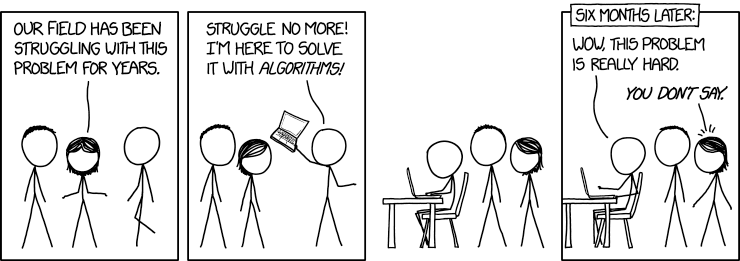
\includegraphics[width=\linewidth]{Figures/Computation/here_to_help}
\caption[Naive use of data mining and computation][Usage naïf de la fouille de données]{On naive use of data mining and intensive computation\label{fig:computation:xkcd}}{De l'usage naïf de la fouille de données et du calcul intensif. Source: \texttt{xkcd}\label{fig:computation:xkcd}}
\end{figure}
%%%%%%%%%%%%%%









%----------------------------------------------------------------------------------------


%%%%%%%%%%%%%%%%%%%%%%
%\subsection[Sensitivity to initial conditions][Sensibilité aux conditions initiales]{Statistical Control on Initial Conditions by Synthetic Data Generation}{Contrôle statistique pour les conditions initiales par génération de données synthétiques}
\subsection{Extend sensitivity analyses}{Étendre les analyses de sensibilité}
	
	

%%%%%%%%%%%%%%%%%%%%%%
\subsubsection{Context}{Contexte}


\bpar{
When evaluating data-driven models, or even more simple partially data-driven models involving simplified parametrization, an unavoidable issue is the lack of control on ``underlying system parameters'' (what is a ill-defined notion but should be seen in our sense as parameters governing system dynamics). Indeed, a statistics extracted from running the model on enough different datasets can become strongly biased by the presence of confounding in the underlying real data, as it is impossible to know if result is due to processes the model tries to translate or to a hidden structure common to all data.
}{
Lors de l'évaluation de modèles basés sur les données, ou même de modèles plus simples partiellement basés sur les données impliquant une paramétrisation simplifiée, une issue inévitable est le manque de contrôle sur les ``paramètres implicites du systèmes'' (ce qui n'est pas une notion stricte mais doit être compris dans notre sens comme les paramètres régissant la dynamique). En effet, une statistique issue d'executions du modèle sur un nombre suffisant d'executions peut toutefois rester biaisée, au sens où il est impossible de savoir si les résultats sont dus aux processus que le modèle cherche à traduire ou à une structure présente dans les données initiales. La question méthodologique fondamentale qui nous intéressera pour la suite est d'être capable d'isoler les effets propres aux processus du modèles de ceux liés à la géographie.
}



\paragraph{Rationale}{Contexte}


\bpar{
Although simulation models of geographical systems in general and agent-based models in particular represent a fantastic opportunity to explore socio-spatial behaviours and to test a variety of scenarios for public policy, the validity of generative models is uncertain until their results are proven robust. Sensitivity analysis usually include the analysis of the effect of stochasticity on the variability of results, as well as the effects of small parameter changes. However, initial spatial conditions are usually taken for granted in geographical models, thus leaving completely unexplored the effect of spatial arrangements on the interaction of agents and of their interactions with the environment. In this part, we present a method to assess the effect of initial spatial conditions on simulation models, using a systematic generator controlled by meta-parameter to create density grids used in spatial simulation models. We show, with the example of a very classical agent-based model (Sugarscape model of ressource allocation) that the effect of space in simulation is significant, and sometimes even larger than parameters themselves. We do so using high performance computing in a very simple and straightforward open-source workflow. The benefits of this approach are various but include for example the knowledge of model behavior in an extended frame, the possibility of statistical control when regressing model outputs, or a finer exploration of model derivatives than with a direct approach.
}{
Bien que les modèles de simulation des systèmes géographiques en général et les modèles basés-agent en particulier représentent une opportunité considérable d'explorer les comportements socio-spatiaux et de tester une variété de scenarios pour les politiques publiques, la validité des modèles génératifs est incertaine tant que la robustesse des résultats n'a pas été établie. Les analyses de sensibilité incluent généralement l'analyse des effets de la stochasticité sur la variabilité des résultats, ainsi que les effets de variations locales des paramètres. Cependant, les conditions spatiales initiales sont généralement prise pour données dans les modèles géographiques, laissant ainsi totalement inexploré l'effet des motifs spatiaux sur les interactions des agents et sur leur interaction avec l'environnement. Dans cette partie, nous présentons une méthode pour établir l'effet des conditions spatiales initiales sur les modèles de simulation, utilisant un générateur systématique contrôlé par des meta-paramètres pour créer des grilles de densité utilisées dans les modèles de simulation spatiaux. Nous montrons, avec l'exemple d'un modèle agent très classique (le modèle Sugarscape d'extraction de ressources) que l'effet de l'espace dans les simulations est significatif, et parfois plus grand que l'effet des paramètres eux-mêmes. Nous y arrivons en utilisant le calcul haute performance en un workflow très simple et open source. Les bénéfices de notre approche sont variés mais incluent par exemple la connaissance du comportement du modèle dans un contexte plus large, la possibilité de contrôle statistique pour régresser les sorties du modèles, ou une exploration plus fine des dérivées du modèle que par rapport à une approche directe.
}



%%%%%%%
%%% - not useful -

%\paragraph{Formalization}{Formalisation}

%\bpar{
%Let first give an abstract formulation of the idea. The generator is considered as an upstream model, coupled simply (outputs become inputs) with the studied downstream model. If $M_u$ is the upstream model, $M_d$ the downstream model and $\alpha$ the meta-parameters, one has the composition of the derivative along the meta-parameter
%\[
%\partial_{\alpha}\left[M_u \circ M_d\right] = \left(\partial_{\alpha} M_u \circ M_d \right)\cdot \partial_{\alpha} M_d
%\]
%It implies that the sensitivity of the downstream model to meta-parameters can be determined by studying the serial coupling and the upstream model. We gain some thematic knowledge, in the sensitivity to an implicit meta-parameter, but there is also a computational gain: the generation of controlled differentiates in the ``initial space'' would be complicated to achieve directly. The question of stochasticity in such simply coupled models causes no additional issue as $\Eb{X}=\Eb{\Eb{X|Y}}$. It naturally multiplies the number of repetition needed for convergence what is the expected behavior.
%}{
%Commençons par donner une formulation abstraite de l'idée, d'un point de vue du couplage de modèle. Le générateur est considéré comme un modèle amont, couplé simplement (les sorties devenant les entrées) avec le modèle aval étudié. Si $M_u$ est le model amont, $M_d$ le modèle aval et $\alpha$ les meta-paramètres, on a la composition de la dérivée le long des meta-paramètres
%\[
%\partial_{\alpha}\left[M_u \circ M_d\right] = \left(\partial_{\alpha} M_u \circ M_d \right)\cdot \partial_{\alpha} M_d
%\]
%Cela implique que la sensibilité du modèle aval aux meta-paramètres peut être déterminée en étudiant le couplage séquentiel et le modèle amont. Nous gagnons de la connaissance thématique, dans la sensibilité à un meta-paramètre implicite, mais il y a aussi un gain computationnel : la génération de différentielles contrôlées dans l'espace initial (c'est-à-dire tester directement la comparaison entre deux grilles proches) serait compliquer à atteindre directement. La question de la stochasticité dans de tels modèles couplés simplement ne pose pas de problème supplémentaire puisque $\Eb{X}=\Eb{\Eb{X|Y}}$. Cela multiplie naturellement le nombre de répétitions pour converger bien évidemment. Nous resterons dans l'application pratique ici à une étude de l'espace faisable de sortie et non à une étude différentielle, cette considération théorique n'influe pas à cet ordre, mais doit être gardée à l'esprit pour d'éventuelles applications plus fines.
%}



\paragraph{The role of spatio-temporal path dependencies}{Role de la dépendance au chemin spatio-temporelle}


\bpar{
Spatio-temporal path dependancy is one of the main reasons making our approach relevant. Indeed, a crucial aspect of most spatio-temporal complex systems is their non-ergodicity~(\cite{pumain2012urban}) (the property that cross-sectional samples in space are not equivalent to samples in time to compute statistics such as averages), what witnesses generally strong spatio-temporal path-dependencies in their trajectories. Similar to what Gell-Mann calls \emph{frozen accidents} in any complex system~\cite{gell1995quark}, a given configuration contains clues on past bifurcations, that can have had dramatic effects on the state of the system. Temporal and cumulative effects have been considered in various geographical subfields and at various geographical scales, including transportation and urban economics, urban geography, and interregional migrations\cite{White1977},\cite{White1978}, \cite{AllenSanglier1979},\cite{Wilson1981},\cite{Pumainetal1989},\cite{AllenSanglier1981},\cite{WeidlichHaag1988},\cite{Portugali2000},\cite{Wilson2002},\cite{batty2007cities},\cite{AzizAlaouiBertelle2009}. Less studied is the impact of the spatial setting on models dynamics and potential bifurcations.
}{
La dépendance au chemin spatio-temporelle est une des raisons principales rendant notre approche pertinente. En effet, un aspect crucial de la plupart des systèmes complexes spatio-temporels est leur non-ergodicité~\cite{pumain2012urban} (la propriété que les échantillons dans l'espace ne sont pas équivalent aux échantillons dans le temps pour calculer des statistiques comme la moyenne), qui témoigne généralement de forte dépendances au chemin spatio-temporelles dans les trajectoires. De manière similaire à ce que \noun{Gell-Mann} appelle \emph{frozen accidents} dans tout système complexe~\cite{gell1995quark}, une configuration donnée contient des indices sur les bifurcations passées, qui peuvent avoir eu des effets considérables sur l'état du système. Les effets temporels et cumulatifs ont été considérés dans de nombreux sous-champs géographiques et à différentes échelles géographiques, par exemple les systèmes régionaux~\cite{Wilson1981} ou l'échelle intra-urbaine~\cite{AllenSanglier1979}. L'impact de la configuration spatiale sur les dynamiques du modèle et les bifurcations spatiales a été moins étudié.
}

\bpar{
The example of transportation networks is a good illustration, as their spatial shape and hierarchy is strongly influenced by past investment decisions, technical choices, or political decisions sometimes not rational~(\cite{zembri2010new}). Some aggregated indicators will not take into account positions and trajectories of each agent (such as segregation in the Schelling model) but others, as in the case of spatial patterns of accessibility in a system of cities, fully capture the path-dependency and may therefore be highly dependent of the initial spatial configuration. It is not clear for example what shifted the economical and political capital of France from Lyon to Paris in the early Middle Age, some assumptions being the reconfiguration of trade patterns from South to North of Europe and thus an increased centrality for Paris due to its spatial position: the bifurcation induced by socio-economic and political factors took a deep significance with worldwide repercussions until today when magnified by the spatial configuration.
}{
L'exemple des réseaux de transport est une bonne illustration, car leur forme spatiale et leur hiérarchie est fortement influencée par les décisions d'investissement du passé, les choix techniques, ou des décisions politiques qui ne sont parfois pas rationnelles~\cite{zembri2010new}. Certains indicateurs agrégés ne prendront pas en compte les positions et trajectoires de chaque agent (comme les inégalités totales dans le modèle Sugarscape) mais d'autres, comme dans le cas des motifs d'accessibilité spatiale dans un système de villes, capture entièrement la dépendance au chemin et peuvent ainsi être fortement dépendants à la configuration spatiale initiale. Il n'est pas clair par exemple ce qui a causé la transition de la capitale française de Lyon à Paris dans le bas Moyen-Age, certaines hypothèses étant la reconfiguration des motifs commerciaux du Sud au Nord de l'Europe et donc une centralité accrue pour Paris due à sa position spatiale, tout en gardant à l'esprit que les centralités géographique et politique ne sont pas équivalentes et entretiennent une relation complexe~\cite{guenee1968espace}. La bifurcation induite par des facteurs socio-économiques et politiques a pris une signification profonde avec des répercussions mondiales encore aujourd'hui quand elle a été concrétisée par la configuration spatiale.
}


\paragraph{Previous attempts in the literature}{Travaux existants}

\bpar{
The effect of the spatial configuration on area-based attributes of human behaviours has been largely discussed in geostatistics, meanly since the exposure of the Modifiable Areal Unit Problem (MAUP) \cite{Openshaw1984},\cite{FotheringhamWong1991}. Recently, \cite{Kwan2012} claims for a careful examination of what she coins the uncertain geographic context problem (UGCoP), that is of the spatial configuration of geographical units even if the size and delineation of the area are the same. On the contrary, the scarcity of these considerations in the geographic simulation model literature questions the generalisation of their results, as it has for instance been showed in the case of LUTI models \cite{Thomasetal2017}, of diffusion processes using ABM \cite{LeTexierCaruso2017}. 
}{
L'effet de la configuration spatiale sur les attributs agrégés à la zone des comportements humains a été largement discuté en géostatistiques, approximativement depuis l'introduction du \emph{Modifiable Areal Unit Problem} (MAUP)~\cite{Openshaw1984}. Plus récemment, \cite{Kwan2012} plaide pour un examen plus attentif de ce qui serait un \emph{Uncertain Geographic Context Problem} (UGCoP), qui est la configuration spatiale des unités géographiques même si la taille et la délimitation des zones est la même. Au contraire, le faible nombre de considérations similaires dans la littérature traitant des modèles de simulation géographiques remet en question la généralisation de leur résultats, comme cela a été montré par exemple dans le cas des modèles LUTI~\cite{Thomasetal2017}, ou des processus de diffusion étudiés par modèles multi-agents~\cite{LeTexierCaruso2017}.
}

%%%%%%%%%%%%%%%%%%%%%%
\subsubsection{Methods}{Méthodes}

\bpar{
In this section, we detail the method developed to analyse the sensitivity of simulation models to initial spatial conditions. In addition to the usual protocol, which consists of running a model $\mu$ with various values of its parameters and relating these variations of values to the variations in the simulation results, we here introduce a spatial generator, which itself is determined by parameters and produces sets of spatial initial conditions. Initial spatial conditions are clustered to represent types of spaces ex-ante (for example: moonocentric or polycentric density grids), and the sensitivity analysis of the model is now run against $\mu$ parameters as well as spatial parameters or spatial types. It allows the sensitivity analysis to produce qualitative conclusions regarding the influence of spatial distribution on the outputs of simulation models, alongside the classic variation of parameter values.
}{
Nous détaillons à présent la méthode développée pour analyser la sensibilité des modèles de simulation aux conditions spatiales initiales. S'ajoutant au protocole usuel, qui consiste à simuler un modèle $\mu$ pour différentes valeurs de ses paramètres et faire le lien entre ces variations aux variations des résultats de simulation, nous introduisons ici un générateur spatial, qui est lui-même déterminé par des paramètres et produit des ensembles de configurations spatiales initiales. Les configurations spatiales initiales sont catégorisées pour représenter des types d'espace typiques (par exemple des grilles de densité monocentriques ou polycentriques), et la sensibilité du modèle est à présent testée sur les paramètres de $\mu$ mais aussi sur les paramètres spatiaux ou les types spatiaux. Cela permet à l'analyse de sensibilité de fournir des conclusions qualitatives au regard de l'influence de la distribution spatiale sur les sorties des modèles de simulation, en parallèle des variation classiques des paramètres.
}

\paragraph{Spatial Generator}{Générateur spatial}


\bpar{
Our spatial generator applies an urban morphogenesis model developed and explored in~\ref{sec:densitygeneration}. To present it in a nutshell, grids are generated through an iterative process which adds a quantity $N$ (population) at each time step, allocating it through preferential attachment characterised by its strength of attraction $\alpha$. This first growth process is then smoothed $n$ times using a diffusion process of strength $\beta$. Grids are thus generated from the combination of the values of these four meta-parameters $\alpha$, $\beta$, $n$ and $N$, in addition to the random seed. To ease our exploration, only the distribution of density is allowed to vary rather than the size of the grid, which we fix to a 50x50 square environment of 100,000 units (cf. figure \ref{fig:spatialGen}).
}{
Le générateur spatial applique un modèle de morphogenèse urbaine développé et exploré en~\ref{sec:densitygeneration}. Pour le présenter rapidement, les grilles sont générées par un processus itératif qui ajoute une quantité de population $N_G$ à chaque pas de temps, l'allouant selon un attachement préférentiel caractérisé par sa force d'attraction $\alpha$. Le premier processus est ensuite lissé $n_d$ fois par un processus de diffusion de force $\beta$. Les grilles sont donc générées aléatoirement par la combinaison des valeurs de ces quatre meta-paramètres $\alpha$, $\beta$, $n_d$ and $N_G$. Pour faciliter l'exploration, seule la distribution de densité est autorisée à varier plutôt que la taille de la grille, qui est fixée à un environnement carré 50x50 de population 100,000 unités.
}




\paragraph{Comparing Phase Diagrams}{Comparer les diagrammes de phase}


\bpar{
In order to test for the influence of spatial initial conditions, we need a systematic method to compare phase diagrams. Indeed, we have as many phase diagrams than we have spatial grids, what makes a qualitative visual comparison not realistic. A solution is to use systematic quantitative procedures. Several potential methods could be used: for example in the case of the Schelling model, an anisotropic spatial segregation index (giving the number of clusters found and in which region in the parameter spaces they are roughly situated) would differentiate strong \emph{meta phase transitions} (phase transitions in the space of meta parameters). The use of metrics comparing spatial distributions, such as the Earth Movers Distance which is used for example in Computer Vision to compare probability distributions~\cite{rubner2000earth}, or the comparison of aggregated transition matrices of the dynamic associated to the potential described by each distribution, would also be potential tools. Map comparison methods, popular in environmental sciences, provide numeral tools to compare two dimensional fields~\cite{visser2006map}. To compare a spatial field evolving in time, elaborated methods such as Empirical Orthogonal Functions that isolates temporal from spatial variations, would be applicable in our case by taking time as a parameter dimension, but these have been shown to perform similarly to direct visual inspection when averaged over a crowdsourcing~\cite{10.1371/journal.pone.0178165}. To keep it simple and as such methodological considerations are auxiliary to the main purpose of this paper, we propose an intuitive measure corresponding to the share of between-diagrams variability relative to their internal variability. More formally, the distance is given by
}{
Afin de tester l'influence des conditions spatiales initiales, nous avons besoin d'une méthode systématique pour comparer des diagrammes de phase. En effet, nous avons autant de diagramme de phase que de grilles spatiales, ce qui rend une comparaison visuelle qualitative non réaliste. Une solution est d'utiliser des procédures quantitatives systématiques. De nombreuses méthodes pourraient potentiellement être utilisées : par exemple, des indicators anisotropes comme la donnée de clusters et leur position dans le diagramme de phase, peuvent permettre de révéler des \emph{meta-transitions de phase} (transition de phase dans l'espace des meta-paramètres). L'utilisation de métriques comparant des distributions spatiales, comme la \emph{Earth Movers Distance} qui est utilisée en vision par ordinateur pour comparer des distributions de probabilité~\cite{rubner2000earth}, ou la comparaison de matrices de transition agrégées de la dynamique associée au potentiel décrit par chaque distribution, est également possible. Les méthodes de comparaison de cartes, répandues en sciences environnementales, fournissent de nombreux outils pour comparer des champs en deux dimensions~\cite{visser2006map}. Pour comparer un champ spatial évoluant dans le temps, des méthodes élaborées comme les Fonctions Orthogonales Empiriques qui isolent les variations temporelles des variations spatiales, seraient applicables dans notre cas en prenant le temps comme une dimension de paramètre, mais celles-ci ont été montrées ayant une performance similaire à la comparaison visuelle directe lorsqu'on prend la moyenne sur un ensemble de contributions crowdsourcées~\cite{10.1371/journal.pone.0178165}. Pour rester simple et car de telles considérations méthodologiques sont auxiliaires pour le propos principal de cette partie, nous proposons une mesure intuitive correspondant à la part de la variabilité inter-diagrammes relativement à leur variabilité interne. Plus formellement, cette distance est donnée par
}

\begin{equation}\label{eq:phase-distance}
d_r\left(\alpha_1,\alpha_2\right) = 2 \cdot \frac{d(f_{\vec{\alpha_1}},f_{\vec{\alpha_2}})^2}{Var\left[f_{\vec{\alpha_1}}\right] + Var\left[f_{\vec{\alpha_2}}\right]}
\end{equation}

\bpar{
where $\alpha \mapsto \left[\vec{x} \mapsto f_{\vec{\alpha}}\left(\vec{x}\right)\right]$ is the operator giving phase diagrams with $\vec{x}$ parameters and $\vec{\alpha}$ meta-parameters, and $d$ is a distance between probability distributions that can be taken for example as basic L2 distance or the Earth's Mover Distance. For each values $\vec{\alpha_i}$, the phase diagram is seen as a random spatial field, facilitating the definition of variances and distance.
}{
où $\alpha \mapsto \left[\vec{x} \mapsto f_{\vec{\alpha}}\left(\vec{x}\right)\right]$ est l'opérateur donnant les diagrammes de phase avec $\vec{x}$ paramètres et $\vec{\alpha}$ meta-paramètres, et $d$ une distance entre distributions de probabilité qui peut être prise par exemple comme la distance L2 basique ou la \emph{Earth Movers Distance}. Pour chaque valeur $\vec{\alpha_i}$, le diagramme de phase est vu comme un champ spatial aléatoire, ce qui facilite la définition des variances et de la distance.
}




%%%%%%%%%%%%%%%%%%%%%%
\subsubsection{Results}{Résultats}


\bpar{
Sugarscape is a model of resource extraction which simulates the unequal distribution of wealth within a heterogenous population (\cite{EpsteinAxtell1996}). Agents of different vision scopes and different metabolisms harvest a self-regenerating resource available heterogeneously in the initial landscape, they settle and collect this resource, which leads some of them to survive and others to perish. The main parameters of this model are the number of agents, their minimal and maximal resource. In addition, we are interested in testing the impact of the spatial distribution of the resource in this project, using the spatial generator. The outcome of the model is measured as a phase diagram of an index of inequality for ressource distribution (Gini index). We extend the implementation with agents wealth distribution of~\cite{li2009netlogo}.
}{
Sugarscape est un modèle d'extraction de ressources qui simule la distribution inégale des richesses dans une population hétérogène~\cite{EpsteinAxtell1996}. Des agents ayant différentes portées de vision et différents métabolismes collectent une ressource qui se régénère automatiquement et disponible de manière hétérogène dans le paysage initial. Ceux-ci s'établissent et collectent la ressource, ce qui mène certains d'entre eux à survivre et d'autres à périr. Les paramètres principaux du modèle sont le nombre d'agents, leur ressources minimale et maximale. Nous nous intéressons principalement à tester l'impact de la distribution spatiale, en utilisant le générateur spatial. La sortie du modèle est mesurée comme le diagramme de phase d'un index d'inégalité pour la distribution de la ressource (index de Gini). Nous étendons l'implémentation ayant initialement une distribution de richesse des agents, donnée par~\cite{li2009netlogo}.
}


\bpar{
For the exploration, 2,500,000 simulations (1000 parameter points x 50 density grids x 50 replications) allow us to show that the model is more sensitive to space than to its other parameters, both qualitatively and quantitatively: the amplitude of variations across density grids is larger than the amplitude in each phase diagram, and the behavior of phase diagram is qualitatively different in different regions of the morphological space. More precisely, we explore a grid of a basic parameter space of the model, which three dimensions are the population of agents $P\in \left[10;510\right]$, the minimal initial agent ressource $s_{-}\in \left[10;100\right]$ and the maximal initial agent ressource $s_{+}\in \left[110;200\right]$. Each parameter is binned into 10 values, giving 1000 parameter points. We run 50 repetitions for each configuration, what yield reasonable convergence properties. The initial spatial configuration varies across 50 different grids, generated by sampling meta-parameters for the generator in a LHS. We did not use the clustered grids to test the flexibility of our framework, which is demonstrated in this case by a direct sequential coupling of the generator and the model. We mesure the distance of all 3-dimensional phase diagrams to the reference phase diagram computed on the default model setup (see Fig.~\ref{fig:sugarscape-distance} for its morphological positioning regarded generated grids), using equation~\ref{eq:phase-distance} with the L2 distance to ensure direct interpretability. Indeed, it gives in that case the average squared distance between corresponding points of the phase diagrams, relative to the average of the variance of each. Therefore, values greater than 1 will mean that inter-diagram variability is more important than intra-diagram variability.
}{
Pour l'exploration, $2.5\cdot 10^6$ simulations (1000 points de paramètres x 50 grilles de densité x 50 réplications) nous permettent de montrer que le modèle est bien plus sensible à l'espace qu'à ses autres paramètres, à la fois quantitativement et qualitativement : l'amplitude des variations entre les grilles de densité est plus grande que l'amplitude dans chaque diagramme de phase, et le comportement de ces diagrammes de phase est qualitativement différent dans diverses régions de l'espace morphologique. Plus précisément, nous explorons une grille d'un espace de paramètre basique du modèle, dont les trois dimensions sont la population des agents $P\in \left[10;510\right]$, la ressource minimale initiale par agent $s_{-}\in \left[10;100\right]$ et la ressource initiale maximale par agent $s_{+}\in \left[110;200\right]$. Chaque paramètre est discrétisé en 10 valeurs, donnant 1000 points de paramètres. Nous procédons à 50 répétitions pour chaque configuration, ce qui donne des propriétés de convergence raisonnables. La distribution spatiale initiale varie parmi 50 grilles initiales, générée en échantillonnant les méta-paramètres du générateur dans un Hypercube Latin. Nous démontrons ainsi la flexibilité de notre cadre, par le couplage séquentiel direct du générateur avec le modèle. Nous mesurons la distance de l'ensemble des diagrammes de phase à 3 dimensions à un diagramme de phase de référence calculé sur l'initialisation du modèle par défaut (voir Fig.~\ref{fig:computation:sugarscape-distance} pour sa position morphologique au regard des grilles générées), en utilisant l'équation~\ref{eq:phase-distance} avec la distance L2 pour assurer une interprétation directe. En effet, cela donne dans ce cas la distance au carré moyenne entre chaque point en correspondance des diagrammes, relative à la moyenne des variances de chaque. Pour cela, des valeurs plus grandes que 1 signifient que la variabilité inter-diagramme est plus importante que la variabilité intra-diagramme.
}


% summary stats
%   Min. 1st Qu.  Median    Mean 3rd Qu.    Max. 
% 0.08909 0.19790 1.52200 1.29600 2.16400 2.98100 

\bpar{
We obtain a very strong sensitivity to initial conditions, as the distribution of the relative distance to reference across grids ranges from 0.09 to 2.98 with a median of 1.52 and an average of 1.30. It means that in average, the model is more sensitive to meta-parameters than to parameters, and the relation variation can reach a factor of 3. We plot in Fig.~\ref{fig:computation:sugarscape-distance} their distribution in a morphological space. The reduced morphological space is obtained by computing 4 raw indicators of urban form, namely Moran index, average distance, rank-size slope and entropy (see~\cite{LeNechet2015} for precise definition and contextualization), and by reducing the dimension with a principal component analysis for which we keep the first two components (92\% of cumulated variance). The first measures a ``level of sprawl'' and of scattering, whereas the second measures aggregation.\footnote{We have $PC1 = 0.76\cdot distance + 0.60\cdot entropy + 0.03\cdot moran + 0.24\cdot slope$ and $PC2 = -0.26\cdot distance + 0.18\cdot entropy + 0.91\cdot moran + 0.26\cdot slope$.} We find that grids producing the highest deviations are the ones with a low level of sprawl and a high aggregation. It is confirmed by the behavior as a function of meta-parameters, as high values of $\alpha$ also yield high distance. In terms of model processes, it shows that congestion mechanisms induce rapidly higher levels of inequality.
}{
Nous obtenons une sensibilité très forte aux conditions initiales, puisque la distribution de la distance relative à la référence s'étend sur l'ensemble des grilles de 0.09 à 2.98, avec un médiane de 1.52 et une moyenne de 1.30. Cela signifie qu'en moyenne, le modèle est plus sensible aux méta-paramètres qu'aux paramètres, et que la variation relative peut atteindre jusqu'à un facteur 3. Nous montrons en Fig.~\ref{fig:computation:sugarscape-distance} leur distribution dans un espace morphologique. L'espace morphologique réduit est obtenu en calculant 4 indicateurs bruts de forme urbaine, qui sont l'index de Moran, la distance moyenne, le niveau de hiérarchie et l'entropie (voir la section~\ref{sec:staticcorrelations} pour une définition précise et une mise en contexte), et en réduisant la dimension avec une analyse par composantes principales pour laquelle nous gardons les deux premières composantes (92\% de variance cumulée). La première mesure un ``niveau d'étalement'' et d'éclatement, tandis que la seconde mesure l'agrégation.\footnote{Nous avons $PC1 = 0.76\cdot distance + 0.60\cdot entropy + 0.03\cdot moran + 0.24\cdot slope$ et $PC2 = -0.26\cdot distance + 0.18\cdot entropy + 0.91\cdot moran + 0.26\cdot slope$.} Nous trouvons que les grilles produisant les déviations les plus grandes sont celles avec un faible niveau d'étalement et une forte agrégation. Cela est confirmé par le comportement comme fonction des meta-paramètres, puisque des fortes valeurs de $\alpha$ donnent aussi une forte distance. En terme de processus du modèle, cela montre que les mécanismes de congestion induisent rapidement de plus haut niveaux d'inégalités.
}

% pca of morphological space
% "","PC1","PC2","PC3","PC4"
%"distance",0.762358566609464,-0.260991693298744,0.200656405132039,0.557162237616392
%"entropy",0.601306167355116,0.181706245959277,0.0958379422351422,-0.772158547261002
%"moran",0.0311129390452153,0.912155429075071,0.30114271129527,0.276256268103684
%"slope",0.237217819823539,0.258531718397015,-0.927289147645628,0.130475642169329

%%%%%%%%%%%%%
\begin{figure}
%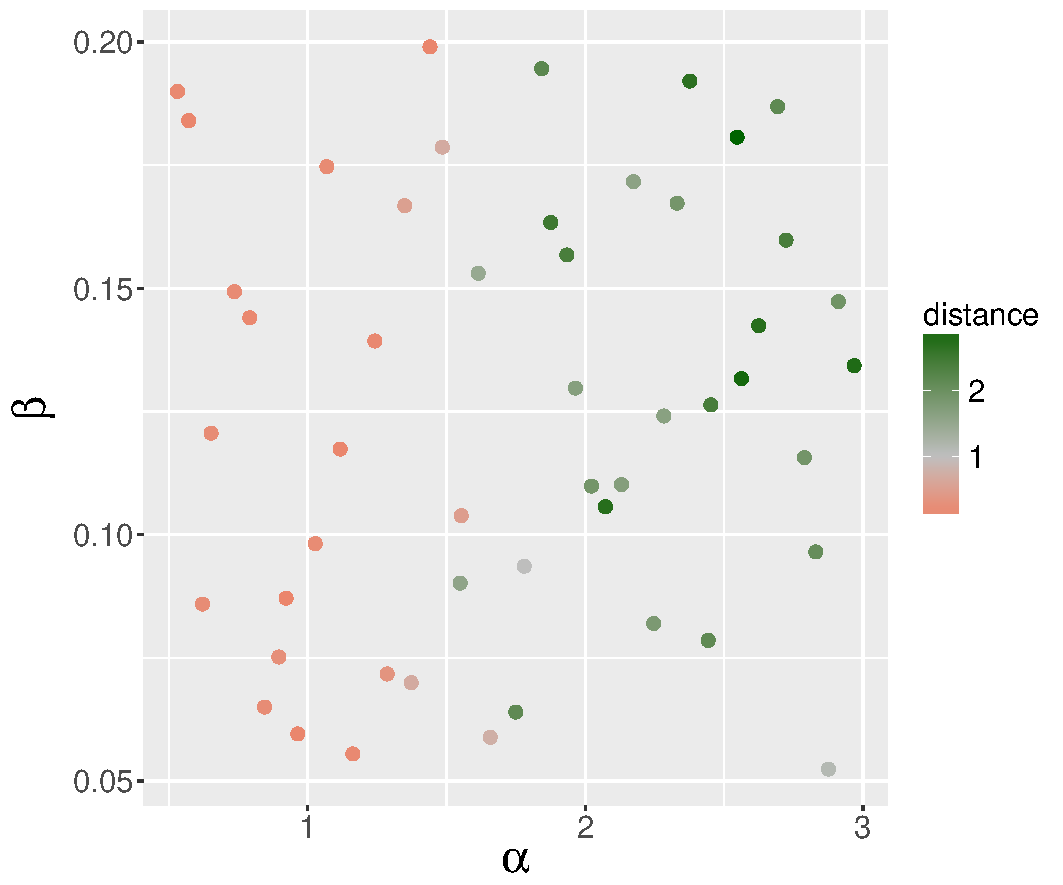
\includegraphics[width=0.49\linewidth]{Figures/Computation/relativedistance_metaparams}
%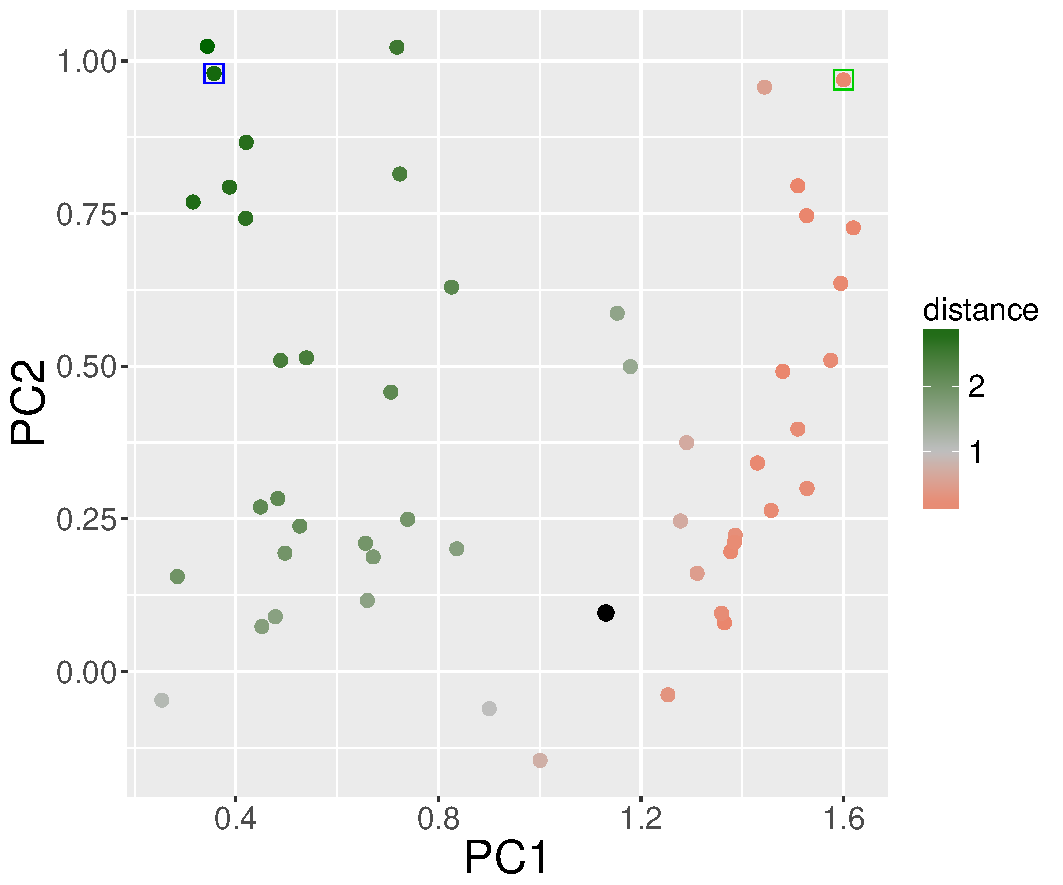
\includegraphics[width=0.49\linewidth]{Figures/Computation/relativedistance_morphspace}
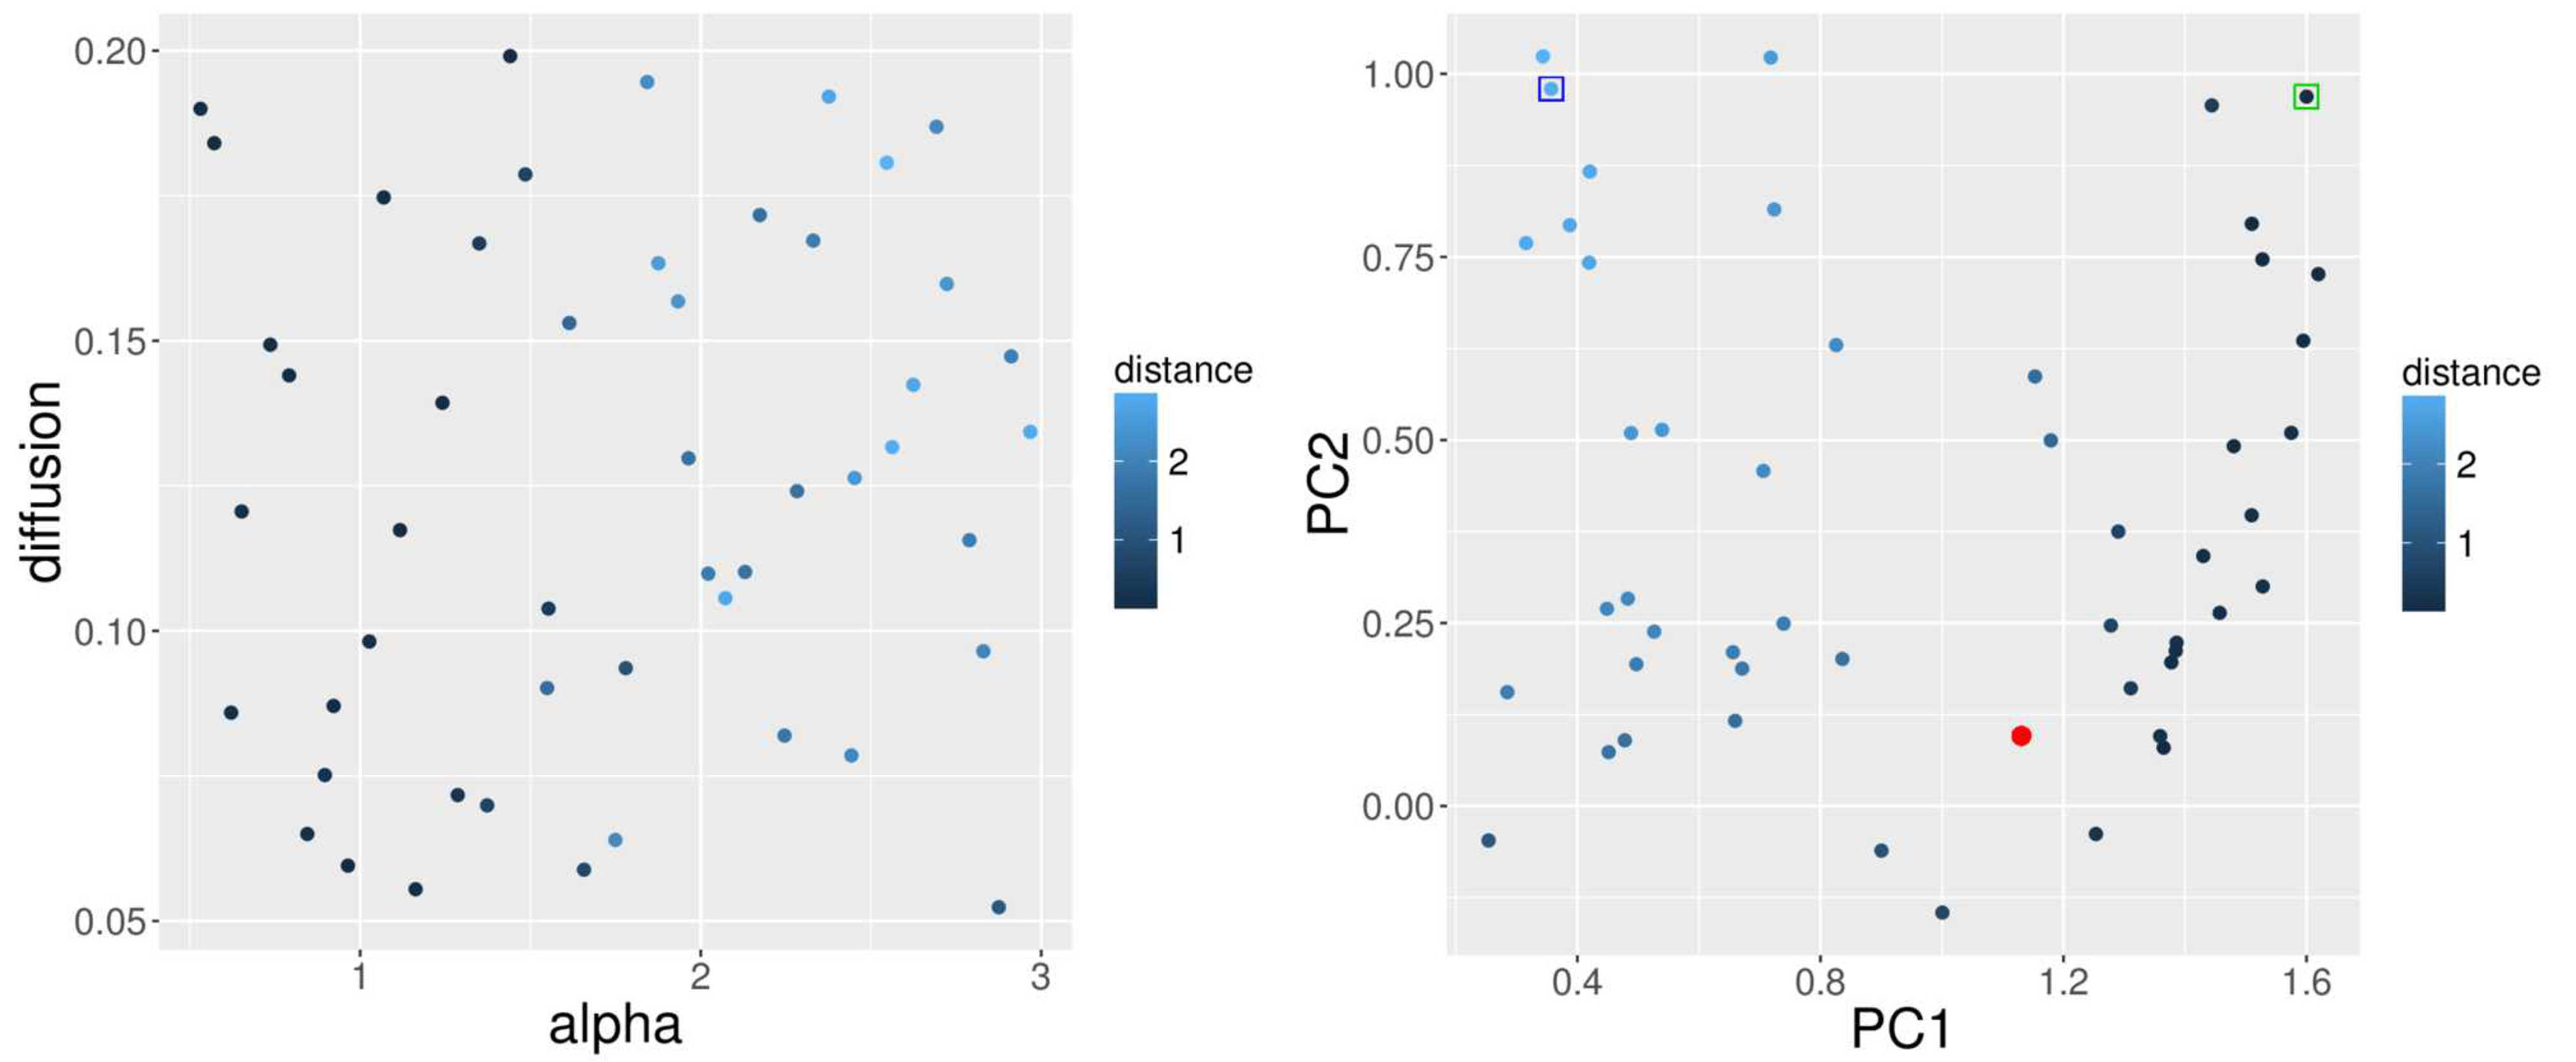
\includegraphics[width=\linewidth]{Figures/Final/3-1-3-fig-computation-sugarscape-distance.jpg}
\caption[Relative distances of phase diagrams to the reference][Distance des diagramme de phase à la référence]{\textbf{Relative distances of phase diagrams to the reference across grids.} (Top) Relative distance as a function of meta-parameters $\alpha$ (strength of preferential attachment) and diffusion ($\beta$, strength of diffusion process). (Bottom) Relative distance as a function of two first principal components of the morphological space (see text). Red point correspond to the reference spatial configuration. Green frame and blue frame give respectively the first and second particular phase diagrams shown in Fig.~\ref{fig:computation:sugarscape-phasediagrams}.\label{fig:computation:sugarscape-distance}}{\textbf{Distance relative des diagrammes de phase à la référence pour l'ensemble des grilles.} (Gauche) Distance relative comme fonction des meta-paramètres $\alpha$ (force de l'attachement préférentiel) et la diffusion ($\beta$, force du processus de diffusion). (Droite) Distance relative comme fonction des deux composantes principales de l'espace morphologique (voir texte). Le point rouge correspond à la configuration spatiale de référence. Les cadres verts et bleu donnent respectivement le premier et le second diagrammes particuliers montrés à la Fig.~\ref{fig:computation:sugarscape-phasediagrams}.\label{fig:computation:sugarscape-distance}}
\end{figure}
%%%%%%%%%%%%%



% phase diagrams -> ok well different qualitatively
%          spAlpha spDiffsteps spDiffusion spGrowth spPopulation
% id=27 : 0.7913103    2.376837   0.1440293 157.4147 4852.746
% id=0 : 2.562398    3.753032   0.1316788 128.4632 4753.983
% maxSugar = 110


%%%%%%%%%%%%%
\begin{figure}
%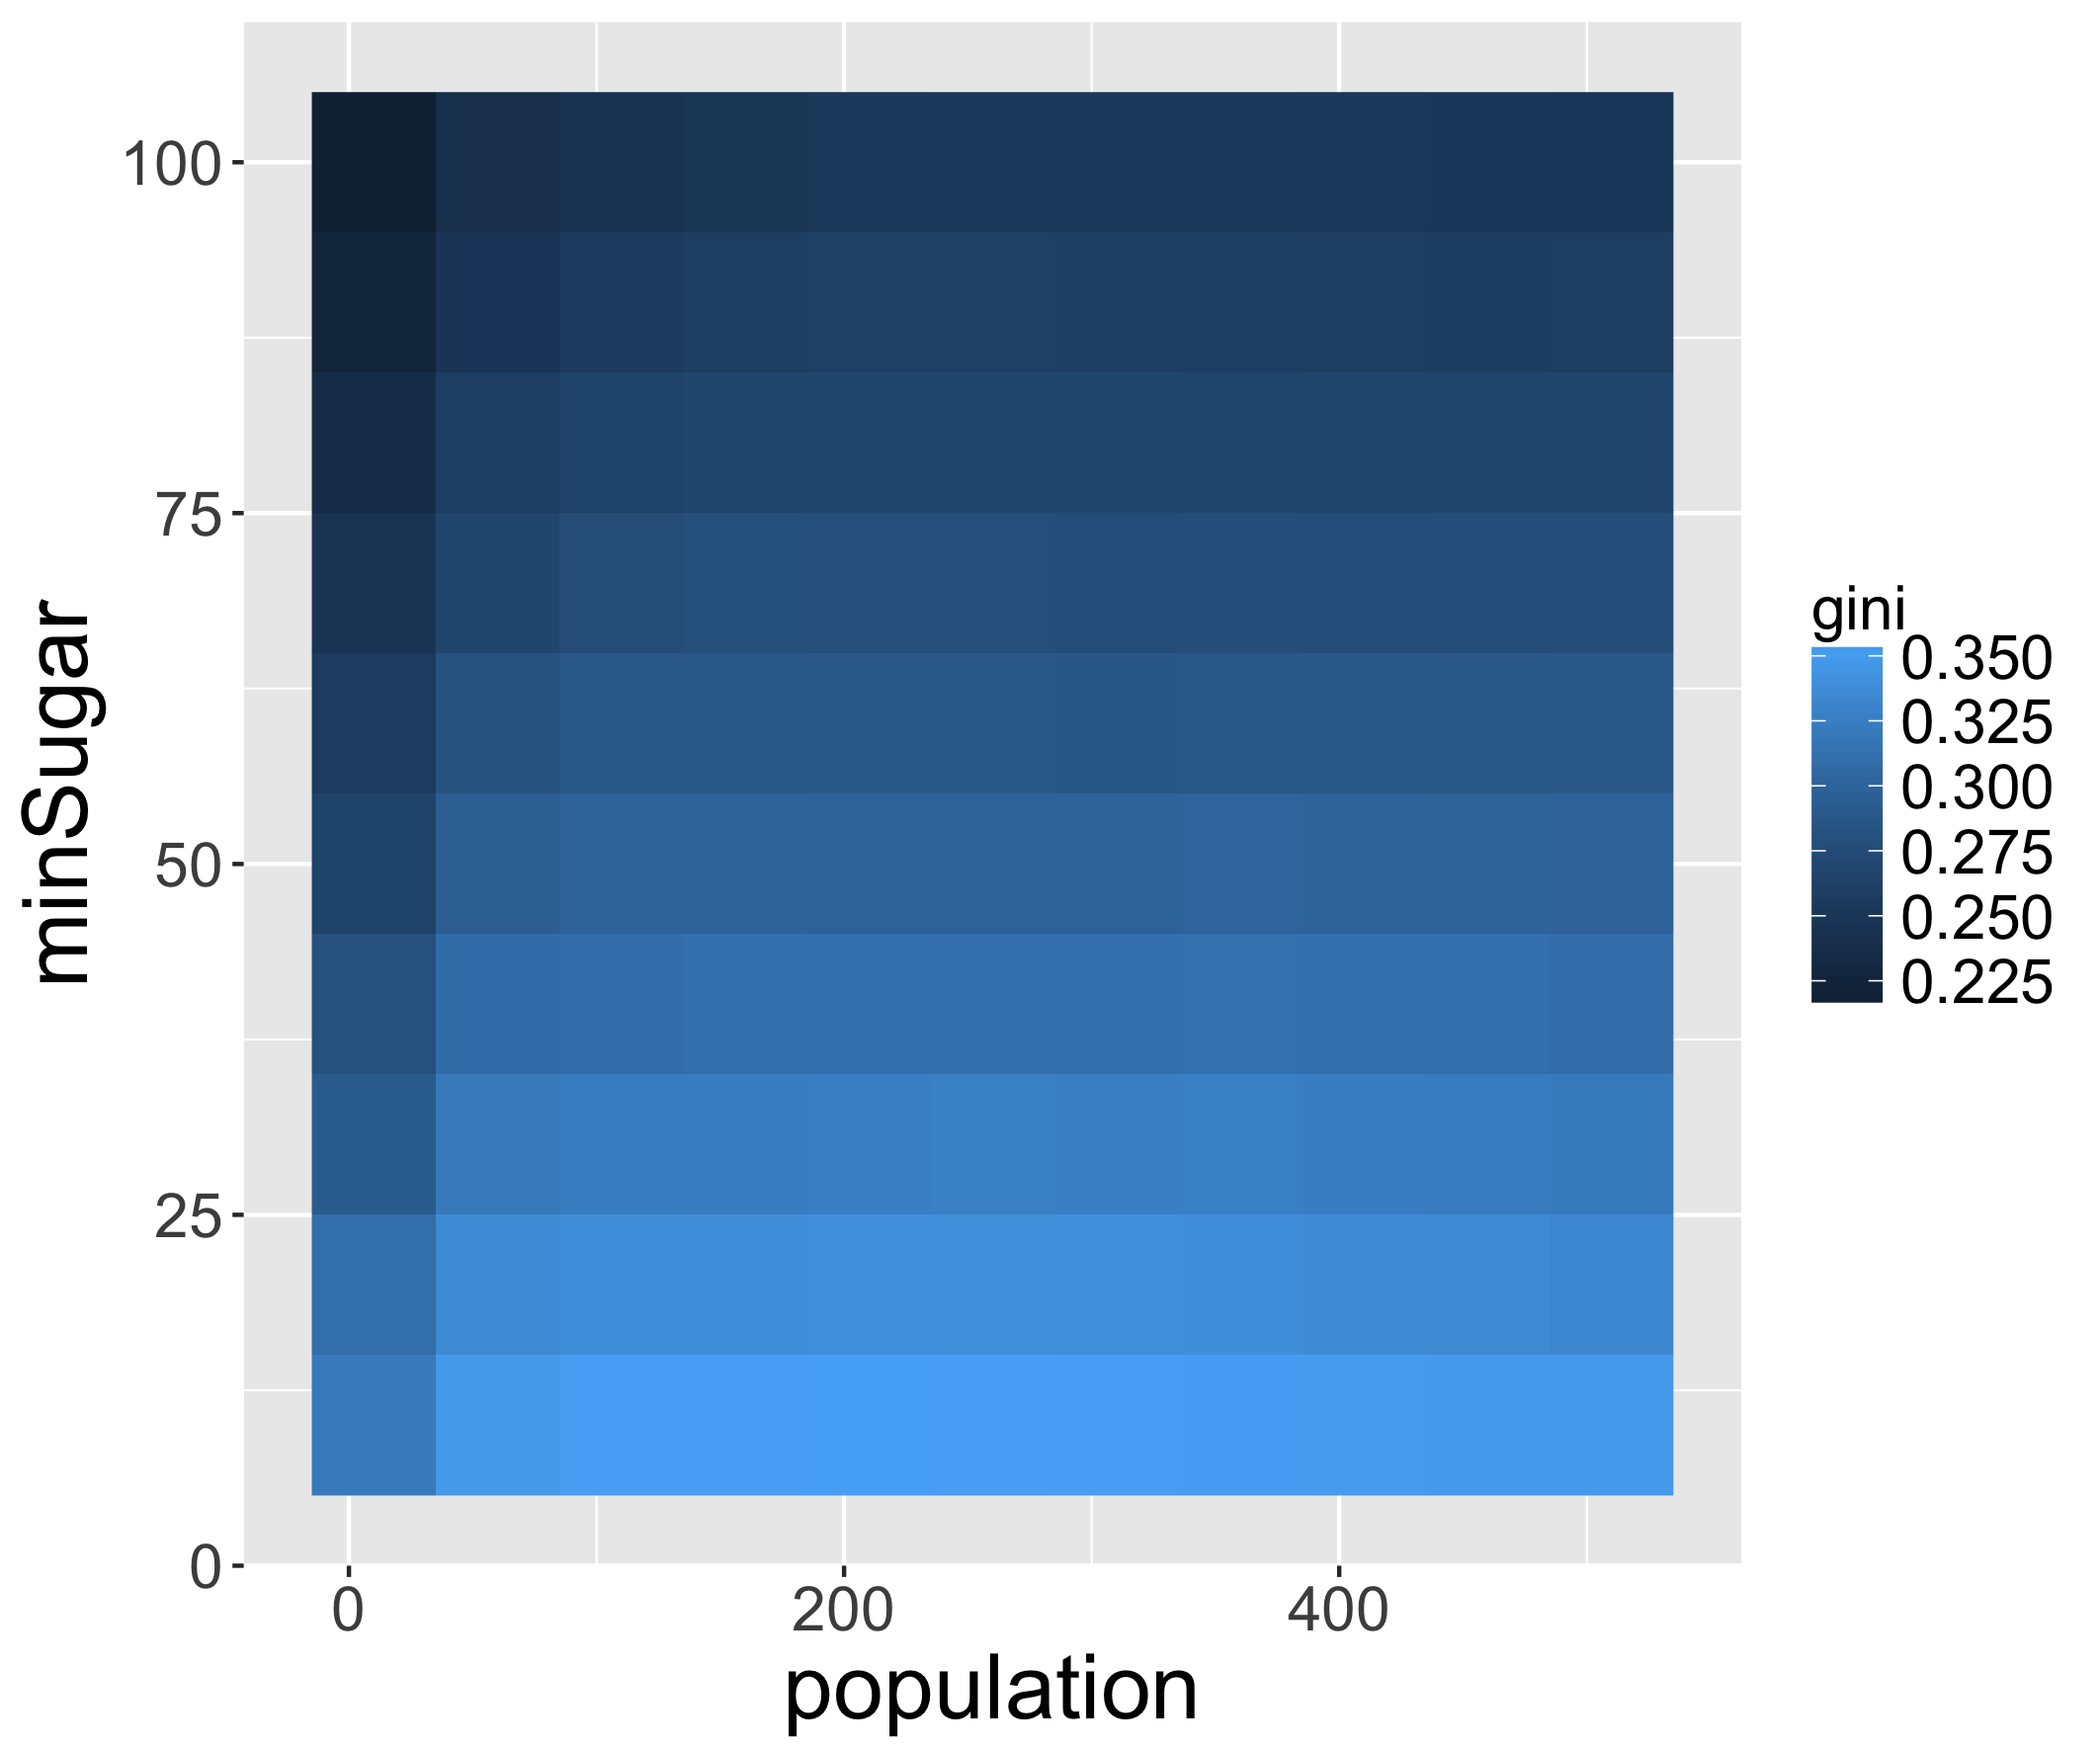
\includegraphics[width=0.49\linewidth]{Figures/Computation/phasediagram_id27_maxSugar110}
%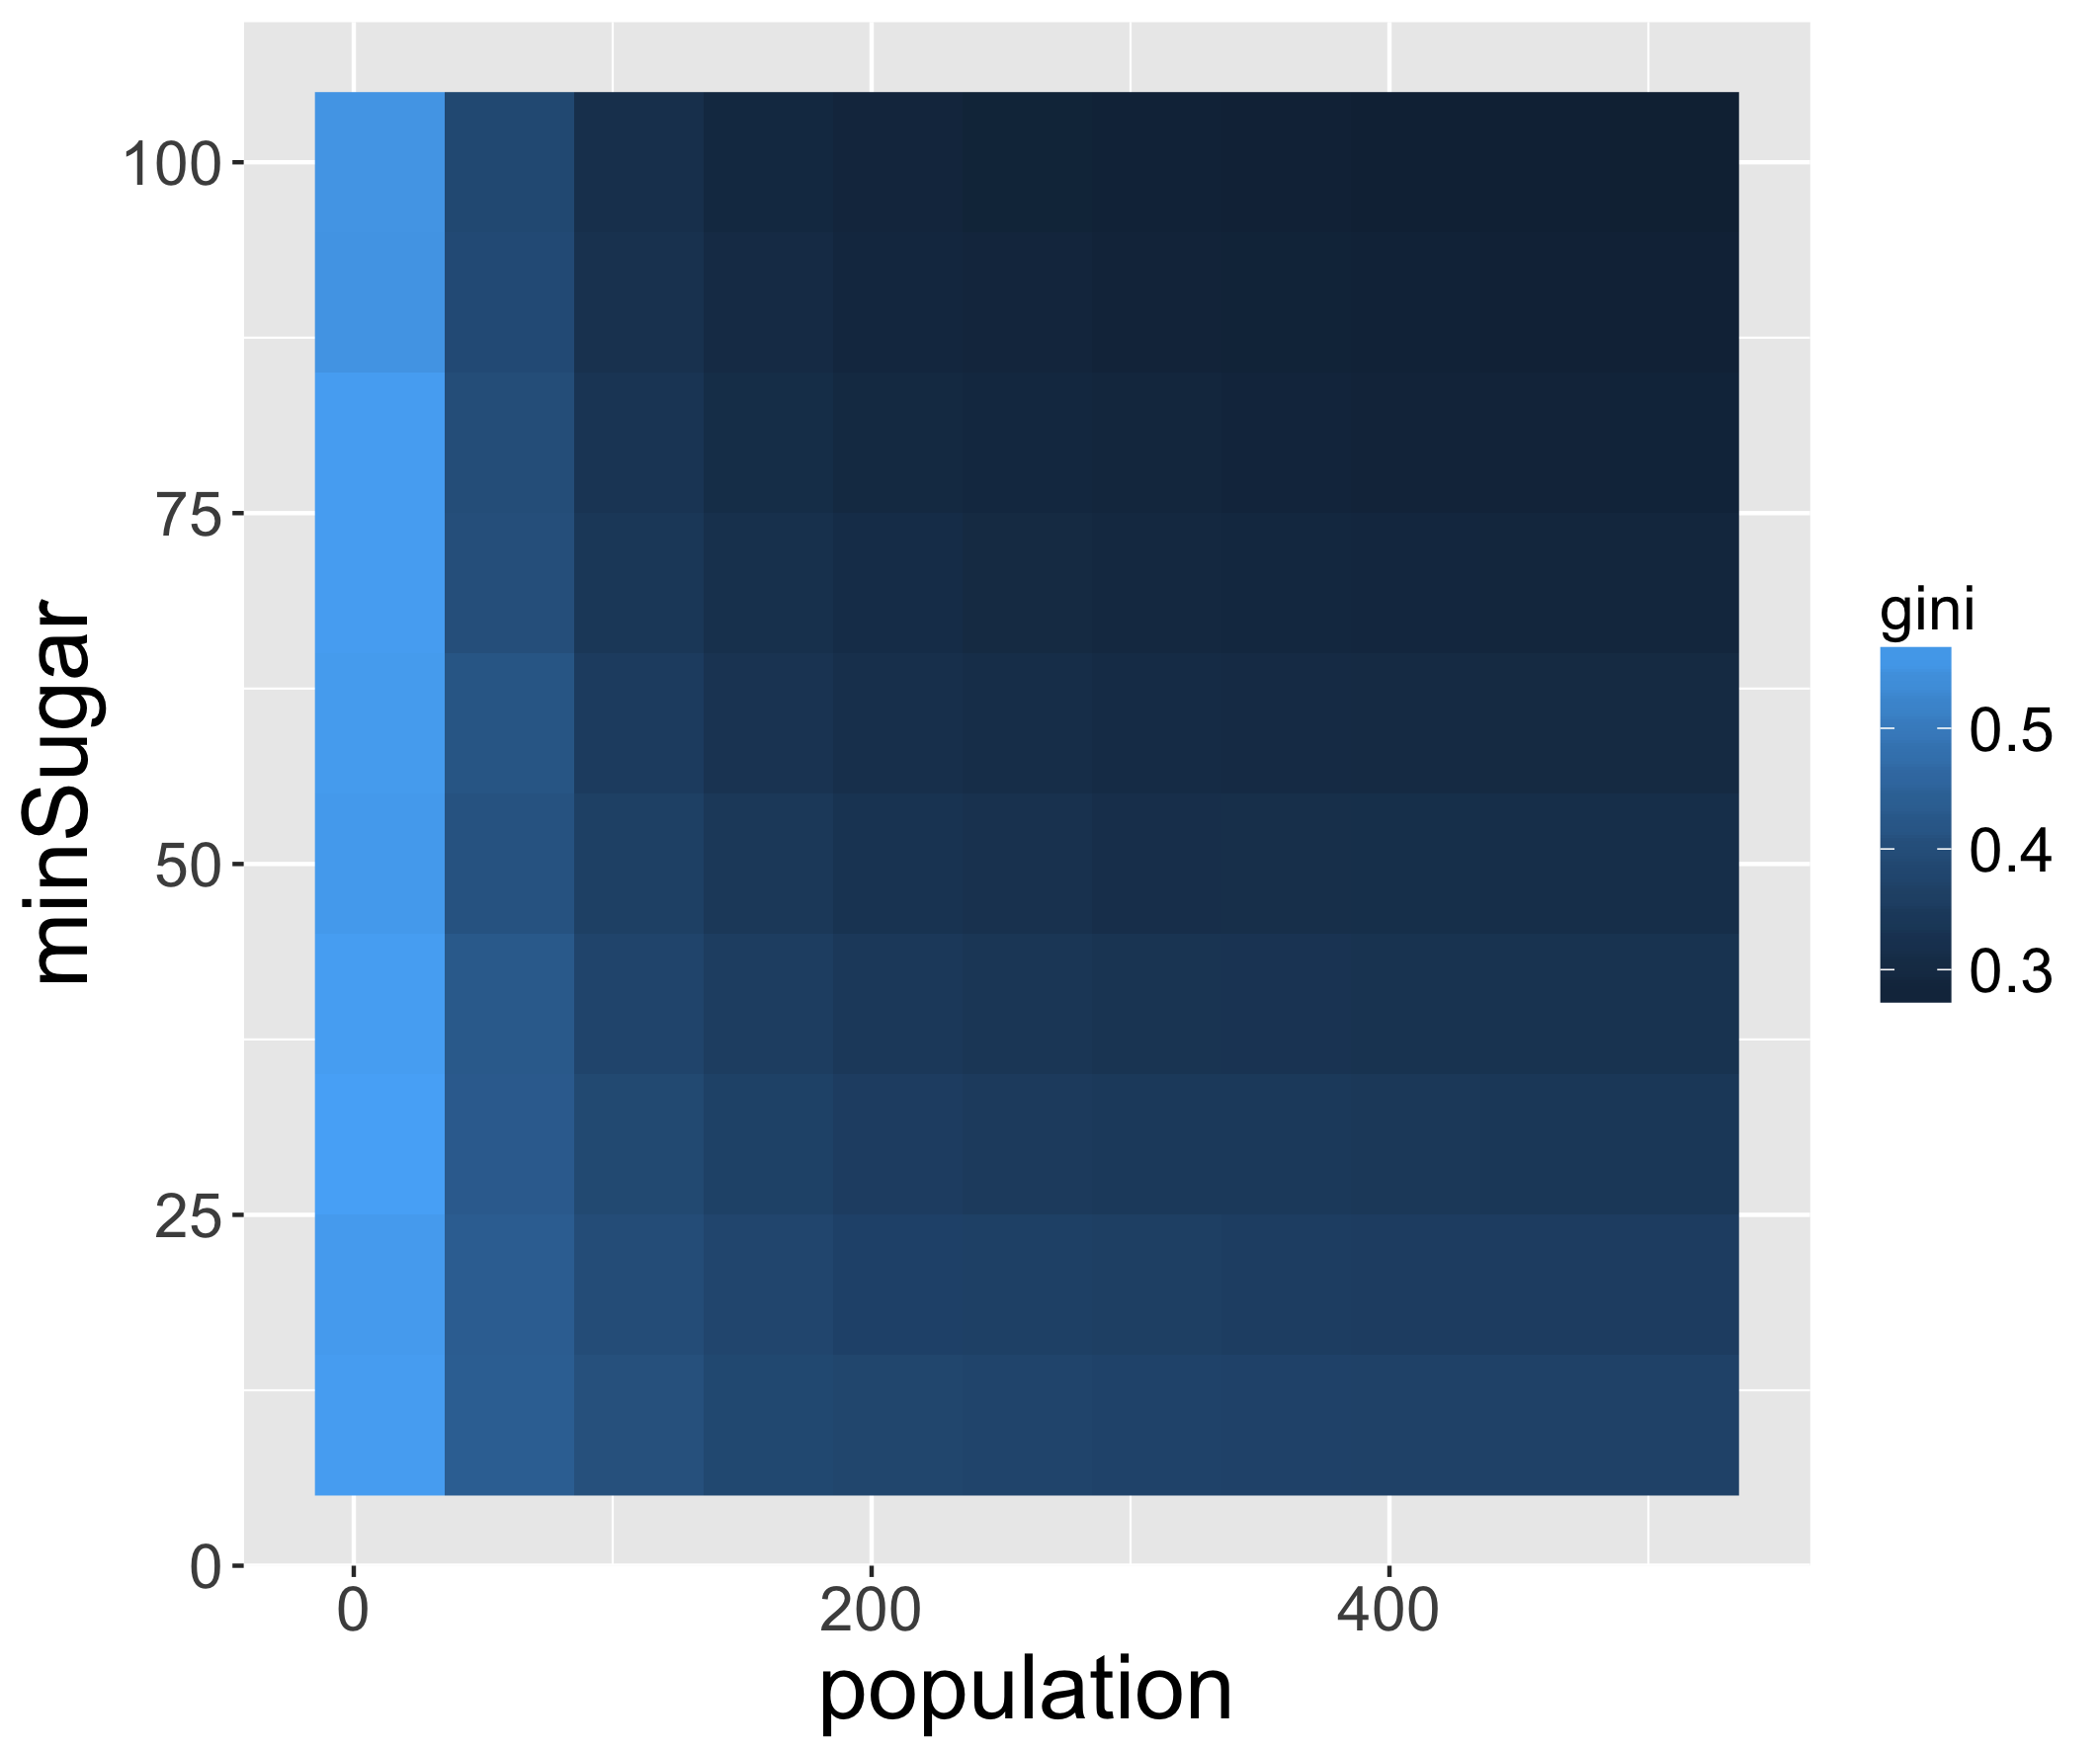
\includegraphics[width=0.49\linewidth]{Figures/Computation/phasediagram_id0_maxSugar110}
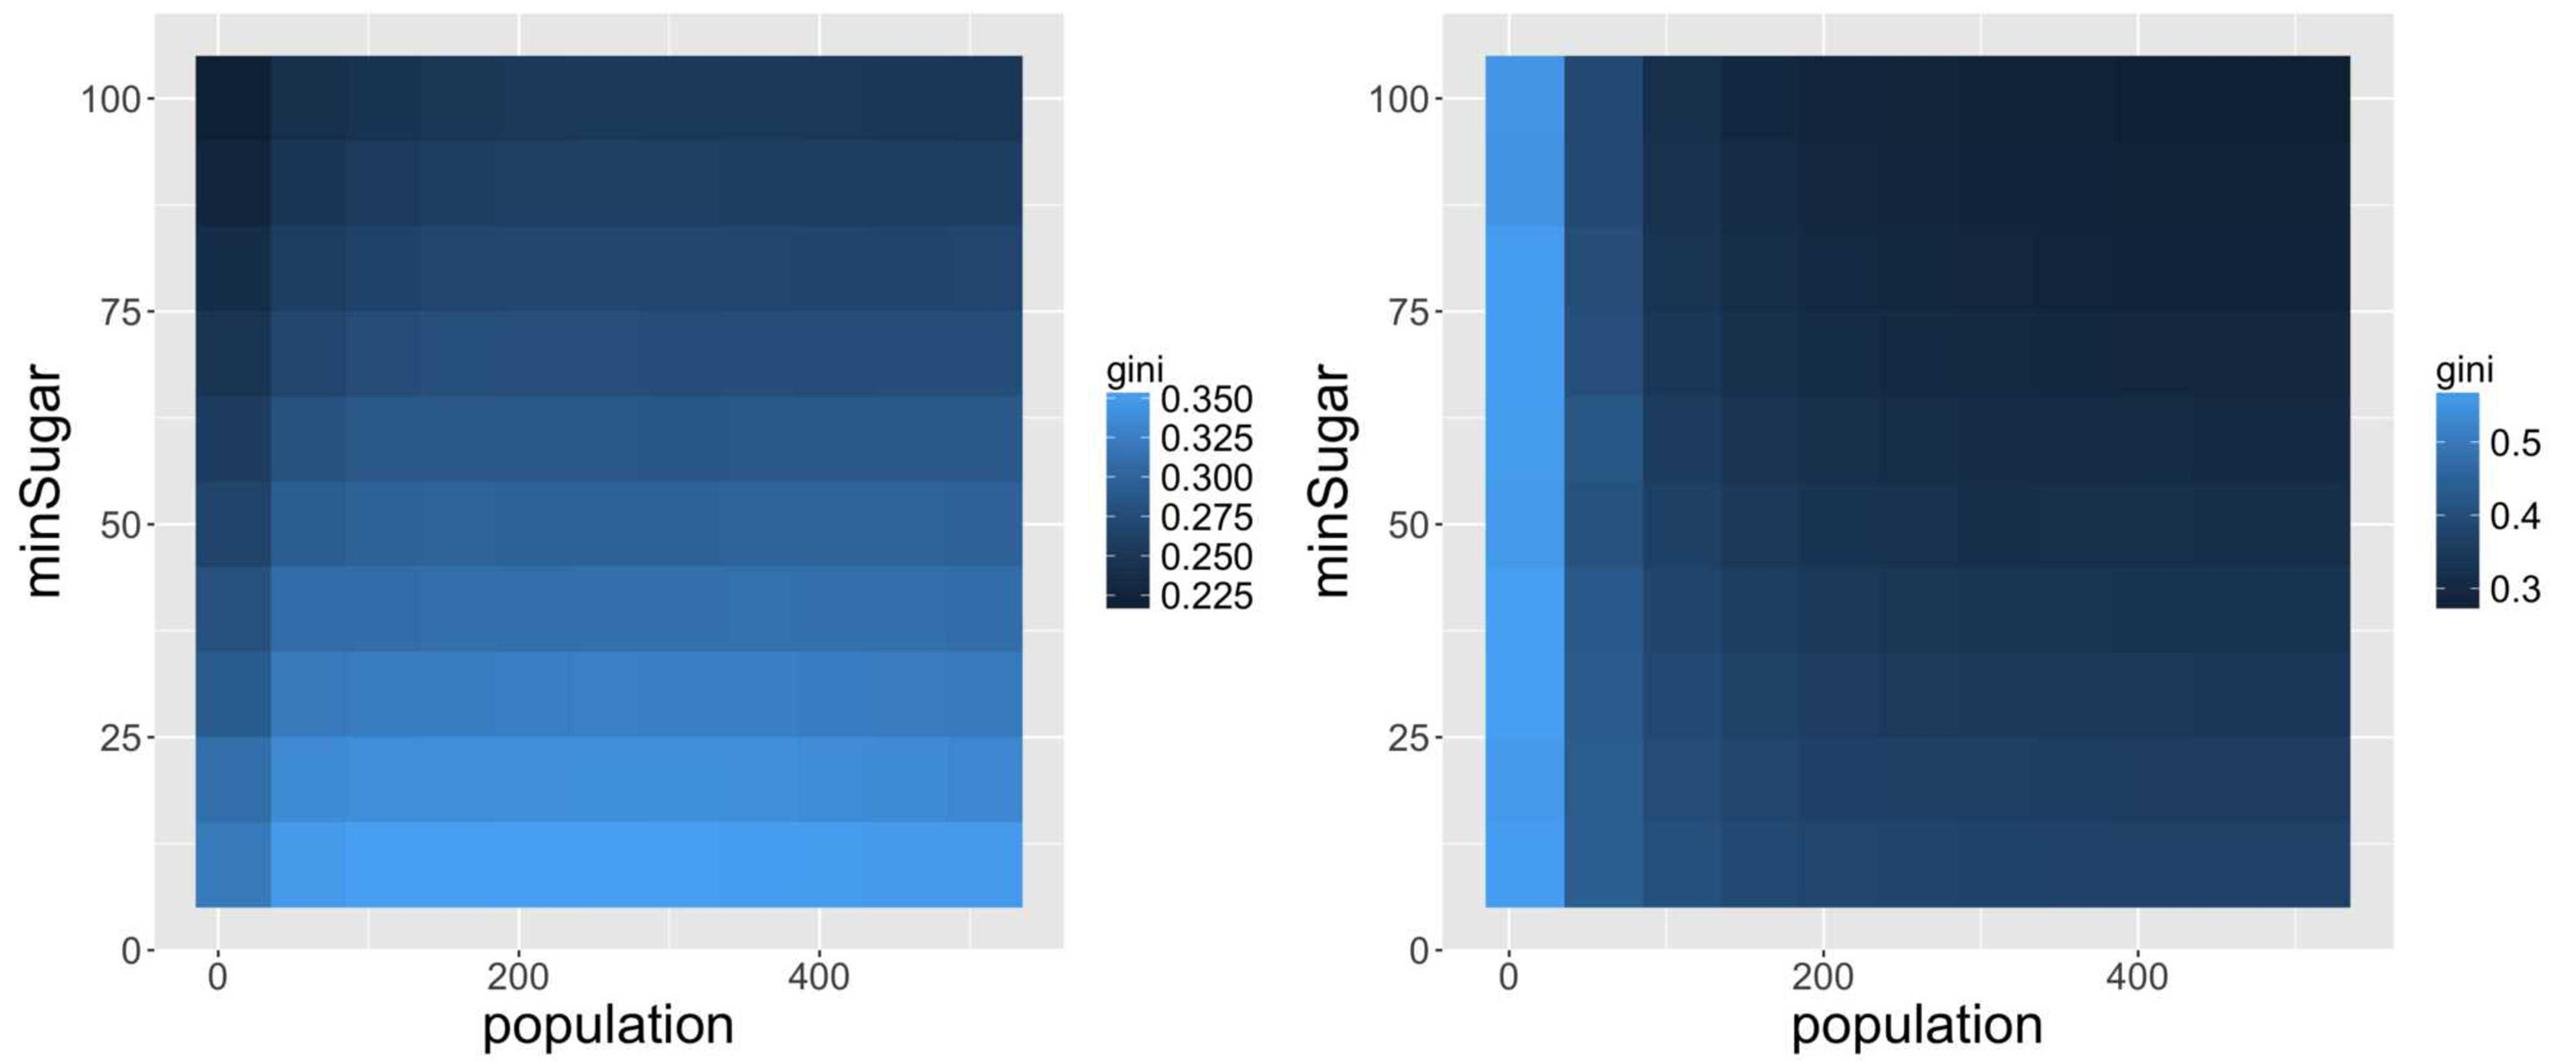
\includegraphics[width=\linewidth]{Figures/Final/3-1-3-fig-computation-sugarscape-phasediagrams.jpg}
\caption[Examples of phase diagrams][Exemples de diagrammes de phase]{\textbf{Examples of phase diagrams.} We show two dimensional phase diagrams on $(P,s_-)$, both at fixed $s_+ = 110$. (Left) Green frame, obtained with $\alpha = 0.79$, $n=2$, $\beta = 0.14$, $N=157$; (Right) Blue frame, obtained with $\alpha = 2.56$, $n=3$, $\beta = 0.13$, $N=128$.\label{fig:computation:sugarscape-phasediagrams}}{\textbf{Exemples de diagrammes de phase.} Nous montrons deux diagrammes bi-dimensionnels sur $(P,s_-)$, obtenus à $s_+ = 110$ fixé. (Gauche) Cadre vert, obtenu avec $\alpha = 0.79$, $n=2$, $\beta = 0.14$, $N=157$ ; (Droite) Cadre bleu, obtenu avec $\alpha = 2.56$, $n=3$, $\beta = 0.13$, $N=128$.\label{fig:computation:sugarscape-phasediagrams}}
\end{figure}
%%%%%%%%%%%%%


\bpar{
We now check the sensitivity in terms of qualitative behavior of phase diagrams. We show the phase diagrams for two very opposite morphologies in term of sprawling, but controlling for aggregation with the same $PC2$ value. These correspond to the green and blue frames in Fig.~\ref{fig:computation:sugarscape-distance}. The behaviors are rather stable for varying $s_+$, what means that the poorest agents have a determinant role in trajectories. The two examples have not only a very distant baseline inequality (the ceil of the first 0.35 is roughly the floor of the second 0.3), but their qualitative behavior is also radically opposite: the sprawled configuration gives inequalities decreasing as population decreases and decreasing as minimal wealth increases, whereas the concentrated one gives inequalities strongly increasing as population decreases and also decreasing with minimal wealth but significantly only for large population values. The process is thus completely inverted, what would have significant impacts if one tried to schematize policies from this model. This second example confirms thus the importance of sensitivity of simulation models to the initial spatial conditions.
}{
Nous contrôlons à présent la sensibilité en terme de comportement qualitatif des diagrammes de phase. Nous montrons en Fig.~\ref{fig:computation:sugarscape-phasediagrams} les diagrammes pour deux morphologies très opposées en terme d'étalement, mais en contrôlant l'agrégation par la même valeur de $PC2$. Ceux-ci correspondent au cadres vert et bleu en Fig.~\ref{fig:computation:sugarscape-distance}. Les comportements sont relativement stables pour $s_+$ variant, ce qui signifie que les agents les plus pauvres ont un rôle déterminant dans les trajectoires. Les deux examples ont non seulement une inégalité de base très distante (le plafond du premier 0.35 est environ le plancher du second 0.3), mais leur comportement qualitatif est également radicalement opposé : la configuration étalée donne des inégalités qui décroissent quand la population décroît et qui décroissent quand la richesse minimale augmente, tandis que la concentrée donne des inégalités augmentant fortement quand la population décroît et aussi décroissantes avec la richesse minimale mais significativement seulement pour des grandes valeurs de population. Le processus est ainsi complètement inversé, ce qui aurait un impact déterminant si l'on essayait de schématiser des politiques à partir du modèle. Cet exemple confirme ainsi l'importance de la sensibilité des modèles de simulation aux conditions spatiales initiales.
}







\stars


Nous avons vu dans cette section comment nous positionner par rapport à l'usage des modèles de simulation, et plus généralement par rapport au calcul intensif. Nous avons vu revenir de manière récurrente dans les problématiques abordées la question de l'ouverture des pratiques scientifiques.

Nous proposons dans la section suivante d'en détailler un aspect, celle de la reproductibilité, qui en est à la fois une composante mais aussi un produit : simultanément produit et producteur, elle permet une plus grande ouverture et est réciproquement encouragée par les pratiques d'ouverture.



\stars


